\documentclass[UTF8,a4paper,8pt]{ctexbook} 

 \usepackage{graphicx}%学习插入图
 \usepackage{verbatim}%学习注释多行
 \usepackage{booktabs}%表格
 \usepackage{geometry}%图片
 \usepackage{amsmath}
 \usepackage{amssymb}
 \usepackage{listings}%代码
 \usepackage{xcolor}  %颜色
 \usepackage{enumitem}%列表格式
 \usepackage{tcolorbox}
 \usepackage{algorithm}  %format of the algorithm
 \usepackage{algorithmic}%format of the algorithm
 \usepackage{multirow}   %multirow for format of table
 \usepackage{tabularx} 	%表格排版格式控制
 \usepackage{array}	%表格排版格式控制
 \usepackage{hyperref}
 \CTEXsetup[format+={\flushleft}]{section}


\geometry{left=1.6cm,right=1.8cm,top=2cm,bottom=1.7cm} %设置文章宽度

\pagestyle{plain} 		  %设置页面布局
\author{\kaishu 郑华}
\title{\heiti 网络编程 笔记}
  %代码效果定义
  \definecolor{mygreen}{rgb}{0,0.6,0}
  \definecolor{mygray}{rgb}{0.5,0.5,0.5}
  \definecolor{mymauve}{rgb}{0.58,0,0.82}
  \lstset{ %
  	backgroundcolor=\color{white},   % choose the background color
  	basicstyle=\footnotesize\ttfamily,        % size of fonts used for the code
  	%stringstyle=\color{codepurple},
  	%basicstyle=\footnotesize,
  	%breakatwhitespace=false,         
  	%breaklines=true,                 
  	%captionpos=b,                    
  	%keepspaces=true,                 
  	%numbers=left,                    
  	%numbersep=5pt,                  
  	%showspaces=false,                
  	%showstringspaces=false,
  	%showtabs=false,        
  	columns=fullflexible,
  	breaklines=true,                 % automatic line breaking only at whitespace
  	captionpos=b,                    % sets the caption-position to bottom
  	tabsize=4,
  	commentstyle=\color{mygreen},    % comment style
  	escapeinside={\%*}{*)},          % if you want to add LaTeX within your code
  	keywordstyle=\color{blue},       % keyword style
  	stringstyle=\color{mymauve}\ttfamily,     % string literal style
  	frame=single,					%tb top and bottom; L left double line
  	xleftmargin=.04\textwidth, 
  	%xrightmargin=.1\textwidth,
  	rulesepcolor=\color{red!20!green!20!blue!20},
  	% identifierstyle=\color{red},
  	language=c++,
  }

\begin{document}          %正文排版开始
 	\maketitle
 	\tableofcontents
 	 
\chapter{进程与线程篇}
	\section{进程、线程-比对}
 	 每个人都有自己的记忆(Memory),人与人通过谈话(消息传递)来交流,谈话即可以面谈(同一台服务器),也可以电话里谈(不同的服务器、有网络通信)。面谈和电话谈的区别在于,面谈可以立即知道对方是否死了,而电话谈只能通过周期性的心跳来判断对方是否还活着。
 	 
 	 有了这些比喻,设计分布式系统时可以采取“角色扮演”,团队里的几个人各自扮演一个进程,人的角色由进程的代码决定(管登陆的、管消息分发的、管买卖的等)。每个人有自己的记忆,但不知道别人的记忆,要想知道别人的看法,只能通过交谈(暂不考虑共享内存这种方式),然后就可以思考:
 	 
	 	\begin{itemize}
		 	\item \textbf{容错}:万一有人突然死了
		 	\item \textbf{扩容}:新人中途加进来
		 	\item \textbf{负载均衡}:把甲的活儿挪给乙做
		 	\item \textbf{退休}:甲要修复Bug,先别派新任务,等他做完手上的事情就把他重启
	 	\end{itemize} 	
	 等等场景,十分便利。
	 
	 线程的特点是共享地址空间,从而可以高效的共享数据。 一台机器上的多个进程能高效的共享代码段,但不能共享数据。如果多个进程大量共享内存,等于是把多进程程序当成多线程来写,掩耳盗铃。		 	

\chapter{TCP/IP 基础篇}    

	\section{层次结构与关系}	
		\subsection{OSI-ISO 7层模型}
				\begin{figure}[h]
					\centering
					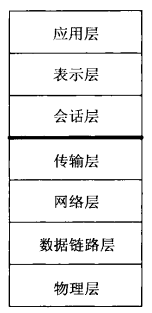
\includegraphics[scale = 0.8]{OSI-Model.png}
				\end{figure}
			
			当然,每个层有每个层的功能,每个对等层之间传输的单位是PDU(propoal  Data Unit),也有每个对等层之间的协议(\textit{如:应用与应用的协议}),具体功能见下:
			\begin{enumerate}
				\item \textbf{应用层:}提供应用程序间通信,\underline{\textbf{A}pplication-PDU},\textit{应用层与应用程序界面沟通,以达到展示给用户的目的。在此常用的协议有\textbf{HTTP},HTTPS,\textbf{FTP},TELNET,SSH,\textbf{SMTP},POP3等}
				\item \textbf{表示层:}处理数据格式、数据加密等,\underline{\textbf{P}resentation-PDU},\textit{对网络传输的数据进行交换,使得多个主机之间传送的信息能够互相理解,包括数据的压缩、加密、格式转换等}
				\item \textbf{会话层:}建立、维护和管理会话,\underline{\textbf{S}ession-pdu},\textit{管理主机之间会话过程,包括会话建立、终止和绘画过程中的管理}
				\item \textbf{传输层:}建立端到端链接,\underline{Segment},\textit{提供可靠的数据传输服务,它检测路由器丢弃的包,然后产生一个重传请求,能够将乱序收到的数据包重新排序}
				\item \textbf{网络层:}寻址和路由选择,\underline{数据包Packet},\textit{负责将各个子网之间的数据进行路由选择,分组与重组,属于本层的协议有IP,IPX,RIP,ICMP,IGMP等,实际使用中的设备如路由器属于本层}
				\item \textbf{数据链路层:}介质访问,链路管理,,\underline{帧Frame},\textit{对物理层的比特流进行数据成帧。提供可靠的数据传输服务,实现无差错数据传输,属于本层的规范有SDLC,PPP,STP,帧中断等,实际使用中的设备如switch交换机属于本层}
				\item \textbf{物理层:}比特流传输,\underline{比特Bit},\textit{定义所有电子及设备的规范,为上层的传输提供一个物理介质,属于本层的协议有RJ-45等,实际使用的设备如网卡等属于本层}
			\end{enumerate}	
			
		\subsection{TCP 4层模型 与 OSI 7层模型 的关系}
			\begin{figure}[h]
				\centering
				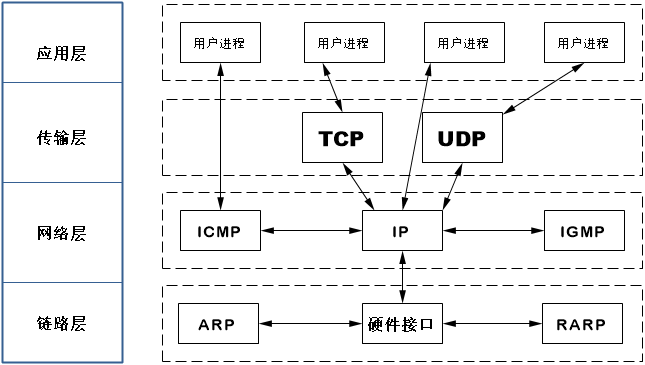
\includegraphics[scale = 0.8]{TCP-4.png}
			\end{figure}
			 \begin{enumerate}
			 	\item \textbf{应用层:}由OSI的\textbf{应用层、表示层、会话层}组成,\textit{用户进程s,ftp,telnet,qq 等}
			 	\item \textbf{传输层:}由OSI的\textbf{传输层}组成,\textit{协议包括TCP,UDP}
			 	\item \textbf{网络层:}由OSI的\textbf{网络层}组成,\textit{协议包括ICMP,IP,IGMP}
			 	\item \textbf{链路层:}由OSI的\textbf{数据链路层、物理层}组成,\textit{协议包括ARP,RARP}
			 \end{enumerate}
			
		\subsection{端口}
				IP 可以选择中某一个主机,但是如何区分使用该主机的哪个服务就要使用端口了,因为一台机器有多个服务在使用。
				
				端口分类如下:
				\begin{itemize}
					\item \textbf{众所周知的的端口:}从0到1023,\textit{这些端口有IANA分配和控制他们紧密绑定于一些服务,通常这些端口的通讯明确的表明了某种服务的协议,例如:21端口为FTP服务端口}
					\item \textbf{注册端口:}从1024到49151,\textit{不受IANA控制,但是由IANA登记并提供使用情况清单。他们松散的绑定于一些服务,也就是说有许多服务绑定于这些端口,这些端口同样用于许多其他目的。如 1433 MicrosoftSQL 服务端口}
					\item \textbf{动态或私有端口:}从49452 到 65535,\textit{IANA不管这些端口,实际上,机器通常从1024起分配动态端口,但也有例外:SUN的RPC端口从32768 开始}
				\end{itemize}
	
	\section{数据链路层相关知识}
		\subsection{最大传输单元(MTU)/路径(MTU)}
			以太网和IEEE802.3 对数据帧的长度都有限制,其最大值分别是1500 和 1492字节,将这个限制称作最大传输单元MTU(Maximum Transmission Unit).
			
			如果IP层有一个数据报要传,而且\textbf{数据的长度比链路层的MTU还大},那么\textbf{IP层就要进行分片},把数据报分成若干片,这样每一片都小于MTU.
			
			当网络上的两台主机相互进行通信时,两台主机之间要经过多个网络,每个网络的链路层可能有不同的MTU,其中两台通信主机\textbf{路径中的最小MTU}被称作\textbf{路径MTU}.
			
		\subsection{以太网帧格式}
		
		\subsection{ARP-地址解析协议:将IP地址解析到MAC地址}
		
		\subsection{RARP-反地址解析协议:将MAC地址解析到IP地址}
		
	\section{网络(IP)层相关知识}
		\subsection{ICMP}
			ICMP 协议用于传递差错信息、时间、回显、网络信息等控制数据,以广播方式-如 ping。
		\subsection{IP 数据报格式}
		
		\subsection{网际校验和}
		
		\subsection{路由}
	
	\section{传输层 相关知识:TCP/UDP }
		\subsection{TCP}
			\subsubsection{TCP 特点}
				\begin{itemize}
					\item 基于字节流:段、无格式、粘包问题
					\item 面向连接:
					\item 可靠传输:
					\item 缓冲传输:
					\item 全双工:
					\item 流量控制:
				\end{itemize}
			\subsubsection{TCP 报文格式}
				\begin{enumerate}[itemindent = 2em]
					\item 	\textbf{确定哪个服务的} 端口号,包括来源端口与目的端口号
					\item 	\textbf{保证可靠传输的} TCP报文序号 与 TCP确认序号
					\item   \textbf{区别报文类型的} 类型字段,包括URG、ACK、PSH、RST、SYN、FIN
					\item 	\textbf{保证传输流畅性的} 滑动窗口大小
					\item   \textbf{保证数据正确性的} 数据校验和
					\item   如果存在紧急指针选项,需要紧急指针
					\item   其他附加选项
				\end{enumerate}
			
			\subsubsection{TCP 如何保证可靠性}
				\begin{itemize}
					\item \textbf{应用数据被分割成TCP认为最合适发送的数据块}。这和UDP完全不同,应用程序产生的数据抱长度不变。由TCP传递给IP的信息单位称为报文段(segment).
					
					\item \textbf{超时重传:}当TCP发出一个段后,它启动一个定时器,等待目的端确认收到这个报文段。如果不能及时收到一个确认,将重发这个报文段。
					
					\item 当TCP收到发自TCP连接另一端的数据,它将发送一个确认。这个确认不是立即发送,通常将推迟几分之一秒。
					
					\item \textbf{TCP将保持它首部和数据的校验和,目的是检验数据在传输过程中的任何变化。}如果收到段的校验和有差错,TCP将丢弃这个报文段并且不确认(导致对方超时重传) 
					
					\item TCP 承载于IP数据报来传输,而IP数据报的到达可能会失序,因此TCP报文段的到达也可能会失序,\textbf{TCP将对收到的数据进行重新排序}。
					
					\item IP数据报会发生重复,TCP的接收端必须\textbf{丢弃重复的数据}。
					
					\item \textbf{TCP还能提供流量控制}。TCP连接的每一方都有一定大小的缓冲空间。
				\end{itemize}
		
		\subsection{UDP}
			\subsubsection{滑动窗口协议}
			
			\subsubsection{UDP 特点}
				\begin{itemize}
					\item 无连接
					\item 不可靠
					\item 一般情况下UDP\textbf{更高效}
				\end{itemize}
			\subsubsection{UDP 报文格式}

\chapter{socket编程篇}
	\section{基本概念}
		\subsection{socket}可以看成是 用户进程 与 内核网络协议栈 的 编程接口。
		
			socket 不仅可以用于本机进程间通信,还可以用于网络上不同主机的进程间通信。
			
			所以每个套接口都必须有地址标记,而地址则包含如下特性:
			\begin{itemize}
				\item 地址家族(\verb|sin_family|):对于IPv4协议来说必须是\verb|AF_INET|.
				\item IPv4 地址(\verb|sin_addr|):IP地址
				\item 端口(\verb|sin_port|):IP主机上服务程序占有的端口号
			\end{itemize}

		\subparagraph{通用地址结构}:
			\begin{lstlisting}
	// 通用地址结构
	struct sockaddr{
		uint8_t sin_len;	//整个sockaddr结构体的长度
		sa_family_t sin_family;//指定改地址家族
		char  sa_data[14];	//由sin_family 决定它的形式,共占14个字节
	}			
			\end{lstlisting}
		\subparagraph{IPv4地址结构}:
			\begin{lstlisting}
	// IPv4 地址结构
	struct sockaddr_in{
		uint8_t sin_len;
		sa_family_t sin_family;
		in_port_t sin_port;  //端口号,占2个字节 
		struct in_addr sin_addr;//IP地址,占4个字节
		char sin_zero[8];	//暂不使用,一般将其设置为0,占8个字节
	}			
			\end{lstlisting}
		\subsection{网络字节序}
			\subsubsection{字节序}
				\subparagraph{大端字节序}
					\textbf{最高}有效位(MSB:most Significant Bit)\textbf{存储于最低}内存地址处,\textbf{最低}有效位(LSB:Lowest Significant Bit)\textbf{存储于最高}内存地址处。
					
				\subparagraph{小端字节序}
					最高有效位(MSB:most Significant Bit)存储于最高内存地址处,最低有效位(LSB:Lowest Significant Bit)存储于最底内存地址处。
			\subsubsection{主机字节序}
				不同的主机有不同的字节序,如x86为小端字节序,Motorola 6800 为大端字节序,ARM字节序是可配置的。
				
				可以通过以下程序进行测试本机的主机字节序
				\begin{lstlisting}
	unsigned int x = 0x12345678;
	unsigned char *p = (unsigned char*) &x;
	printf("%0x %0x %0x %0x\n",p[0],p[1],p[2],p[3]);				 
				\end{lstlisting}
			\subsubsection{网络字节序}网络字节序规定为 \textbf{大端字节序}
			
			\subsubsection{字节序转换函数}
				\begin{itemize}
					\item \textit{host to network long 长整数-主机字节序转网络字节序: uint32\_t \textbf{htonl}(uint32\_t hostlong);}
					\item \textit{host to network short:  uint16\_t \textbf{htons}(uint16\_t hostshort);}
					\item \textit{network to host long 长整数-网络字节序转主机字节序:  uint32\_t \textbf{ntohl}(uint32\_t netlong);}
					\item \textit{network to host short:  uint16\_t \textbf{ntohs}(uint16\_t netshort);}
				\end{itemize}
				
			\subsubsection{地址转换函数}
				在机器中地址(00110001010101)一般用32位整数表示,而我们在操作中使用的都为点分式IP(192.168.1.32)地址。所以就涉及一个转换。
				\begin{itemize}
					\item 整数 \textbf{转} 点分IP:\verb|char * inet_ntoa(struct in_addr in);|
					\item 点分IP \textbf{转} 整数:\verb|in_addr_t inet_addr(const char* cp);|// \verb|in_addr_t| 结构体其实就是一个无符号32位整数.
				\end{itemize}
			
		\subsection{套接字类型}
			\begin{itemize}
				\item \textbf{流式套接字}(\verb|SOCK_STREAM|)[TCP]:提供面向连接的、可靠的数据传输服务,数据无差错、无重复的发送、且按发送顺序接受、消息无边界。
				\item \textbf{数据报式套接字}(\verb|SOCK_DGRAM|)[UDP]:提供无连接服务、不提供无错保证、数据可能丢失和重复、并且接受顺序混乱、消息有边界。
			\end{itemize}	
			
		\subsection{流式套接字的粘包问题}
			因为是流式传输,所以消息的格式随意且长度随意即无边界,导致接受方 读取接受信息时可能多读或少读的问题称为粘包问题。
			\subparagraph{产生原因}
				
			\subparagraph{处理方案}
				本质上是要在应用层维护消息与消息的边界:
				
				\begin{itemize}
					\item 定长包:write\_N --> read\_N
					\item 包围加结束标记\verb|\r \n|等
					\item 报文头部包括 信息长度.
				\end{itemize}
		
		\subsection{获取本机网络地址}
			\begin{itemize}
				\item \textit{getsockname(int 套接字描述符, struct sockaddr*(Client的)\textbf{[赋值]}通用地址-即将取出请求的socket的地址赋值给该参数通过指针返回, 地址长度)}:\textbf{获取本地地址-IP、端口}:127.0.0.1-51323;
				\item \textit{gethostname(char *host\textbf{[赋值]},size\_t lenOfHostName)}:获取主机名
				\item \textit{struct hostent* gethostbyname(char *host)}:\textbf{通过主机名返回该主机的网络地址list},ip = hostent->h\_addr\_list[i] 或 host->h\_addr;192.168.23.12、127.0.0.1、127.0.1.1;
			\end{itemize}
			
	\section{基本的C/S 通信模型}
		\subsection{通信模型}
		
		\subsection{客户端使用的函数及作用}
			\begin{itemize}
				\item \textbf{int socket(int 协议族,int TCPorUDPorRaw,int 协议类型)}:类似于电话机,失败返回-1.
				\item \textbf{connect(int 套接字描述符,struct sockaddr*-(Server的)\textbf{[传值]}使用通用地址格式, 地址长度)}:连接请求
				\item \textit{write()}:
				\item \textit{read()}:接受并从缓存区移除消息
				\item \textit{recv()}:接受但不移除缓冲区消息
			\end{itemize}
			\begin{lstlisting}
	int main()
	{
		/*
		申请套接字:申请使用电话机
		*/
		int sockfd;
		if((sockfd = socket(AF_INET, SOCK_STREAM, IPPROTO_TCP)) < 0)
			exit(1);
		
		/*
		明确服务器地址(IP、协议族、端口)
		*/
		struct sockaddr_in serverAddr;
		memset(&serverAddr, 0,sizeof(serverAddr));
		serverAddr.sin_family = AF_INET;
		serverAddr.sin_port = htons(5188);
		serverAddr.sin_addr.s_addr = inet_addr("127.0.0.1");
		
		/*
		连接服务器
		*/
		if((connect(sockfd, (struct sockaddr*)&serverAddr, sizeof(serverAddr)))<0)
			exit(1);
		
		/*
		通信
		*/
		char sendbuf[1024] = {0};
		char recvbuf[1024] = {0};
		while(fgets(sendbuf,sizeof(sendbuf),stdin) != NULL)
		{
			write(sockfd, sendbuf, strlen(sendbuf));
			read(sockfd, recvbuf, sizeof(recvbuf));
			fputs(recvbuf, stdout);
			
			memset(recvbuf, 0, sizeof(recvbuf));
			memset(sendbuf, 0, sizeof(sendbuf));
		}
		return 0;
	}			
			\end{lstlisting}
		\subsection{服务器使用的函数及作用}
			\begin{itemize}
				\item \textbf{socket()}:
				\item \textbf{int bind(int 套接字描述符,struct sockaddr*-使用通用地址格式, 地址长度)}:绑定本地地址到套接字-使用通用类型.包括IP、端口号、协议族。
				\item \textbf{int listen(int 套接字描述符, int 此套接字排队的最大连接个数)}:确定最大的并发数-等价于确认 未完成连接+已完成连接 是否小于 最大并发连接数。
					\begin{itemize}
						\item 未完成连接:未完成3次握手
						\item 已完成连接:完成3次握手
					\end{itemize}
				\item \textbf{int accept(int 套接字描述符, struct sockaddr*(Client的)\textbf{[赋值]}通用地址-即将取出请求的socket的地址赋值给该参数通过指针返回, 地址长度)}:从已完成队列返回第一个连接,如果已连接队列为空,则阻塞
				\item \textit{read()}:
				\item \textit{write()}:
			\end{itemize}
			
			\begin{lstlisting}
	int main()
	{
		/*
		申请套接字:申请使用电话机
		*/
		int listenfd;
		if((listenfd = socket(AF_INET, SOCK_STREAM, IPPROTO_TCP)) < 0)
			exit(1);
		
		/*
		明确服务器地址(IP、协议族、端口)
		*/
		struct sockaddr_in serverAddr;
		memset(&serverAddr, 0,sizeof(serverAddr));
		serverAddr.sin_family = AF_INET;
		serverAddr.sin_port = htons(5188);
		// 确定主机 IP 的3种方式
		/*serverAddr.sin_addr.s_addr = htonl(INADDR_ANY);*/
		/*serverAddr.sin_addr.s_addr = inet_addr("127.0.0.1");*/
		/*inet_aton("127.0.0.1",&serverAddr.sin_addr);*/
		/*
		解决多次调用bind() 产生的TIME_WAIT问题:利用ReuseAddr 
		*/
		int on = 1;
		if(setsockopt(listenfd, SOL_SOCKET, SO_REUSEADDR, &on, sizeof(on)) < 0)
			exit(1);
		
		/*
		绑定本地地址即服务器地址(IP、协议族、端口)到 套接字
		*/
		if(bind(listenfd, (struct sockaddr *)&serverAddr, sizeof(serverAddr)) < 0)
			exit(1);
		
		/*
		确定连接的最大数-即最大并发数
		*/
		if(listen(listenfd, SOMAXCONN) < 0)
			exit(1);// 等待过多
		
		/*
		从已完成队列-取出第一个连接,该套接字将不再处于监听状态
		*/
		struct sockaddr_in peerAddr;
		socklen_t peer_len = sizeof(peerAddr);
		int conn;
		if((conn = accept(listenfd, (struct sockaddr*)&peerAddr, &peer_len))< 0)
			exit(1);
		
		/*
		消息通信
		*/
		// 根据具体应用书写如:
		char recvbuf[1024];
		while(1)
		{
			memset(recvbuf, 0 sizeof(buf));
			read(conn,recvbuf,sizeof(recvbuf));
			fputs(recvbuf,stdout);
			write(conn,recvbuf,strlen(recvbuf));
		}
		
		return 0;
	}			
			\end{lstlisting}
		\subsection{REUSEADDR}
			当本机服务器关闭后立即重启时会存在 Bind错误:Address already use. 因为服务器重启又要绑定地址,这时已经将该端口号绑定给该程序,当改程序关闭时,端口会处在TIME\_WAIT状态- 等待一定时间后才会释放,所以在这个状态下 再绑定 会出现 bind 错误。
			
			\subparagraph{解决方案}实现参考上述代码
			
				\begin{enumerate}
					\item 服务器尽可能使用ReuseAddr
					\item 在绑定(\verb|bind()|)前尽可能调用 \verb|setsockopt| 来设置ReuseAddr 套接字选项。 
					\item 使用ReuseAddr选项可以\textbf{使得不必等待}\verb|TIME_WAIT| \textbf{状态消失就可以重启服务器}。
				\end{enumerate}
				
		\subsection{close与shutdown 的区别}
			\url{http://blog.csdn.net/jnu_simba/article/details/9068059}
			\subparagraph{发送方}
				\verb|send() + shutdown(WR)FIN + read()->0(等待服务器) + close()|
			\subparagraph{接收方}
				\verb|read()->0 + if nothing more to send + close()|
				
			\subparagraph{shutdown 与 close}
				\begin{itemize}[itemindent = 1em]
					\item \verb|shutdown(SD_SEND)|\textbf{先把}\verb|socket|缓冲区中的数据发送出去,\textbf{然后}发送\verb|FIN数据包|,所谓的“从容关闭”,仅仅做这些事,并且这个时候,并没有释放本地资源,也就是,一切皆文件,\verb|socket|在内核分配的资源没有释放,像\verb|File|对象、\verb|Inode|节点,\verb|dentry,file_struct|等等一个文件所对应的资源,\textbf{都没有被释放}。
						\begin{enumerate}[itemindent = 1em]
							\item \verb|SHUT_RD|:\textbf{关闭连接的读端}。也就是该套接字不再接受数据,任何当前在套接字接受缓冲区的数据将被丢弃。进程将不能对该套接字发出任何读操作。对\verb|TCP|套接字该调用之后接受到的任何数据将被确认然后无声的丢弃掉。
							\item \verb|SHUT_WR|:\textbf{关闭连接的写端},进程不能在对此套接字发出写操作 
							\item \verb|SHUT_RDWR|:相当于调用\verb|shutdown|两次:首先是以\verb|SHUT_RD|,然后以\verb|SHUT_WR| 
						\end{enumerate}
					\item \verb|close|会把\verb|socket|缓冲区中的数据先\textbf{马上}丢弃,然后发送\verb|FIN数据包|,所谓的“暴力关闭”并且,关闭本地文件对象,释放资源。
						\begin{enumerate}[itemindent = 1em]
							\item close 把描述符的引用计数减1,仅在该计数变为0时才关闭套接字。
							\item close 终止读和写两个方向的数据传送。
						\end{enumerate}
				\end{itemize}
		
		\subsection{FIN 与 RST}
			\subsubsection{FIN}
				\verb|Socket| 正常情况下 发送的最后一个报文
				
			\subsubsection{RST}
				\verb|RST|表示复位,用来\textbf{异常的关闭连接}。发送\verb|RST|包关闭连接时,\textbf{不必等缓冲区的包都发出去},直接就丢弃缓存区的包发送\verb|RST|包。而\textbf{接收端}收到\verb|RST|包后,\textbf{也不必}发送\verb|ACK|包来确认。
				
				下面列出几种会出现\verb|RST|的情况:\url{https://my.oschina.net/costaxu/blog/127394}
					\begin{enumerate}[itemindent = 1em]
						\item 服务器程序端口未打开而客户端来连接。
						\item 提前关闭
					\end{enumerate}
				
		\subsection{SIGPIPE}
			在接受到对方关闭消息\verb|FIN|时,如果继续向对方发消息,那么对方会返回\verb|RST|段,如果还继续写,那么将产生\verb|SIGPIPE |信号,终止该进程。
			
			处理可以是选择性的:
			
			1- 常规捕捉信号 \verb|signal(SIGPIPE,void handle(int sig))|
			
			2- \textbf{忽略该信号 }\verb|signal(SIGPIPE, SIG_IGN)|,一般情况下 程序启动时忽略\verb|SIGPIPE|信号,防止服务器意外退出。
		
		\subsection{TCP No Delay}
			nagle's 算法等待每一次的确认,造成的延迟问题
			
				解决:buffering , 或disable nagle's 算法(\verb|TCP_NODELAY|)
			
		\subsection{多进程服务器-允许多client访问}
			上述的服务器代码是无法完成多client的访问的,因为accept只取了一次已完成的套接字,所以改进就在此处,而问题并不是 listen 应该创建个线程或进程。
			
			fork 函数要点:fork后,子进程中的文件会从父进程拷贝一份,然而每个文件都有一个引用计数,此时对应的文件就会引用计数加一
			
			close 函数要点:只有socket文件引用计数为0时才会真正的关闭并发送FIN
			\begin{lstlisting}
	void do_service(int conn)
	{
		char recvbuf[1024];
		while(1)
		{
			memset(recvbuf, 0 sizeof(buf));
			int ret = read(conn,recvbuf,sizeof(recvbuf));
			if(ret == 0)
			{
				printf("Client Closed\n");
				break;
			}
			fputs(recvbuf,stdout);
			write(conn,recvbuf,strlen(recvbuf));
		}
	}
	
	int main()
	{
		...
		//  取套接字
		struct sockaddr_in peerAddr;
		socklen_t peer_len = sizeof(peerAddr);
		int conn;
		
		pid_t pid;
		while(1)
		{
			// 从以完成队列中取出第一个套接字
			if((conn = accept(listenfd, (struct sockaddr*)&peerAddr, &peer_len))< 0)
				exit(1);
			// 打印客户端 IP、 端口号
			printf("Client Ip = %s Port = %d\n",inet_ntoa(peerAddr.sin_addr),ntohs(peerAddr.sin_port));
			
			// 为每个新的 Client 分出新的进程处理请求
			pid = fork();
			if(pid == -1)
			exit(1);
			
			// 如果是子进程
			if(pid == 0)
			{
				do_service(conn);
				close(conn);
				exit(EXIT_SUCCESS);
			}
			//  父进程收尾
			else 
			..	
		}
		
		close(listenfd);
		return 0;
	}			
			\end{lstlisting}	
	\section{Peer To Peer 点对点通信:P2P}
		点对点的意思就是:
			\begin{itemize}
				\item 服务器与客户端 都-既可以 发消息 也可以 收消息。
				\item 仍然存在 客户与服务 概念
			\end{itemize}
		\subsection{信号机制}
			发信号与收信号. kill(pid, SIGUSR1) --> signal(SIGUSR1, handle\_func);
			
			\subparagraph{应用}:可以通过发信号的方式通知某个不知道是否该结束的等待进程退出。如下,在P2P的情况下,当 客户端退出时 服务器的 收消息进程知道客户端退出了,但是服务器的发消息进程并不知道客户端退出了,这是需要使用 信号通知发消息进程退出。服务器退出同理。
		
		\subsection{服务器端}
			接受请求并开始点对点通信.
			\begin{lstlisting}
	/*
	信号处理函数
	*/
	void sig_handle_func(int sig)
	{
		printf("Got sig = %d, and Close\n",sig);
		exit(EXIT_SUCCESS);
	}
	
	int main()
	{
		...
		
		if((conn = accept(listenfd, (struct sockaddr*)&peerAddr, &peer_len))< 0)
			exit(1);
		// 打印客户端 IP、 端口号
		printf("Client Ip = %s Port = %d\n",inet_ntoa(peerAddr.sin_addr),ntohs(peerAddr.sin_port));
		
		// 为每个新的 Client 分出新的进程处理请求
		pid = fork();
		if(pid == -1)
			exit(1);
		
		// 如果是子进程:负责发消息
		if(pid == 0)
		{	
			/*
			接收消息
			*/
			signal(SIGUSR1,sig_handle_func);
			
			char sendbuf[1024] = {0};
			while(fgets(sendbuf, sizeof(sendbuf), stdin) != NULL)
			{
				write(conn, sendbuf, strlen(sendbuf));
				memset(sendbuf, 0, sizeof(sendbuf));
			}
			exit(EXIT_SUCCESS);
		}
		//  父进程:负责读消息
		else 
		{
			char recvbuf[1024];
			while(1)
			{
				memset(recvbuf, 0 sizeof(buf));
				int ret = read(conn, recvbuf, sizeof(recvbuf));
				if(ret == 0)
				{
					printf("Client Closed\n");
					break;
				}
				fputs(recvbuf,stdout);
			}
			/*
			发消息
			*/
			kill(pid, SIGUSR1);
			exit(EXIT_SUCCESS);
		}	
		return 0;
	}			
			\end{lstlisting}
		\subsection{客户端}	 
			请求连接,并要求服务器完成点对点服务。
			
			关闭发送消息进程 也是类似于服务器的 消息机制。
	\section{fork 进程}
		\begin{lstlisting}
	#include <unistd.h>   
	#include <stdio.h>    
	int  main ()   
	{   
		pid_t fpid; //fpid表示fork函数返回的值   
		int  count=0;  
		fpid=fork();   
		if  (fpid < 0)   
			printf("error in fork!" );   
			else   if  (fpid == 0) {  
			printf("i am the child process, my process id is %d/n" ,getpid());   
			printf("我是爹的儿子/n" ); //对某些人来说中文看着更直白。   
			count++;  
		}  
		else  {  
			printf("i am the parent process, my process id is %d/n" ,getpid());   
			printf("我是孩子他爹/n" );  
			count++;  
		}  
		printf("统计结果是: %d/n" ,count);  
		return  0;  
	}  
		\end{lstlisting}
		
		\textbf{fork调用}的一个奇妙之处就是它仅仅被调用一次,却能够返回两次,它可能有三种不同的返回值: 
		\begin{enumerate}[itemindent = 2em]
			\item 在父进程中,fork返回新创建子进程的进程ID;
			\item 在子进程中,fork返回0;
			\item 如果出现错误,fork返回一个负值;
		\end{enumerate}
		
		\textbf{fork出错}可能有两种原因:
		\begin{enumerate}[itemindent = 2em]
			\item 当前的进程数已经达到了系统规定的上限,这时errno的值被设置为EAGAIN。
			\item 系统内存不足,这时errno的值被设置为ENOMEM。
		\end{enumerate} 
		 
		 \textbf{fork执行完毕后},出现两个进程,\textbf{作用域代码共享},如下图所示:
			 \begin{figure}[h]
			 	\centering
			 	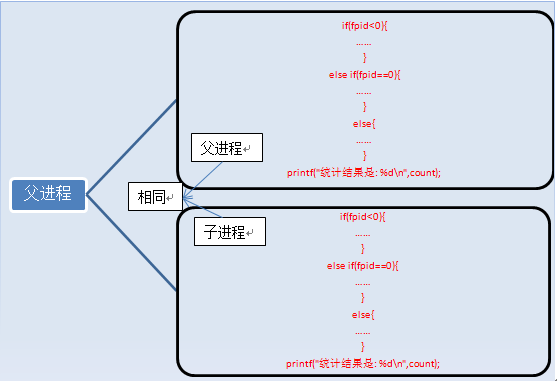
\includegraphics[scale = 0.7]{fork.jpg}
			 \end{figure}
	\section{僵尸进程}
		如果\textbf{子进程}\textit{先于}\textbf{父进程}退出, 同时父进程又没有调用wait/waitpid,则该子进程将成为僵尸进程。
		
		\subsection{参考}
			介绍:\url{http://www.cnblogs.com/yuxingfirst/p/3165407.html}
			
			避免:\url{http://blog.chinaunix.net/xmlrpc.php?r=blog/article&uid=26872853&id=4574069}
			
		\subsection{wait 与 waitpid}
			\url{http://blog.csdn.net/kevinhg/article/details/7001719}
			
			waitpid:父进程利用工作的简短间歇察看子进程的是否退出,如退出就收集它。(相当于管理一个队列)
			
			wait:父进程将自己阻塞,直到有子进程退出为止(相当于等待系统资源)
	\section{孤儿进程}
		一个\textbf{父进程退出},而它的一个或多个\textbf{子进程还在运行},那么那些\textbf{子进程将成为孤儿进程}。孤儿进程将被init进程(进程号为1)所收养,并由init进程对它们完成状态收集工作。
				
	\section{守护进程}
		守护进程是在后台运行且不与任何控制终端相关联的进程。\textbf{通常由}系统初始化脚本启动,当然\textbf{也可以}在shell提示符下用命令行启动,不过\textbf{这种}守护进程\textbf{必须亲自脱离于控制终端的关联}。
		
		\begin{itemize}
			\item \textbf{创建子进程,终止父进程}-变成孤儿进程
			\item 在子进程中创建新会话,调用\verb|setsid|的三个作用:让进程摆脱原会话的控制、让进程摆脱原进程组的控制和让进程摆脱原控制终端的控制。
			\item 改变工作目录
			\item 重设文件创建掩码
		\end{itemize}
		
		\subsection{守护进程的输出}
			\url{http://blog.csdn.net/smstong/article/details/8919803}
			
			由于守护进程没有终端,所以它的消息用\verb|fprintf到stderr|上,从守护进程登记消息使用\verb|syslog|函数,作为替换, 也可以使用\verb|openlog closelog|。
						
			syslog是一种标准的协议,分为客户端和服务器端,客户端是产生日志消息的一方,而服务器端负责接收客户端发送来的日志消息,并做出保存到特定的日志文件中或者其他方式的处理。
			
			在Linux中,常见的syslog的服务器端程序是syslogd守护程序。
			
			\verb|void syslog(int priority,const char *message,…);|
			\begin{itemize}
				\item priority:由level与facility 共同决定
				
					\verb|level ->|
					\begin{itemize}
						\item \verb|LOG_ERR|
						\item \verb|LOG_WARNING|
						\item \verb|LOG_NOTICE|
						\item \verb|LOG_INFO|
					\end{itemize}
					
					\verb|facility ->|
					\begin{itemize}
						\item \verb|LOG_LOCAL1|
						\item \verb|LOG_KERN|
						\item \verb|LOG_DEAMON|
					\end{itemize}
				\item message: 要传递的消息
			\end{itemize}
			
			\verb|example->|
				\verb|syslog(LOG_INFO||\verb|LOG_LOCAL2, "read name(%s,%s)", str, str2);|
		\subsection{守护进程的启动方法有}
			\begin{enumerate}
				\item \textbf{系统初始化阶段,由系统初始化脚本启动}。这些脚本通常位于\verb|/etc、/etc/rc|开头的某个目录中。由这些脚本启动的守护进程从一开始就有\verb|root|特权。例如:inetd超级服务器、Web服务器、邮件服务器、\verb|syslogd|守护进程等都用这种方式启动。
				\item 靠\verb|inetd|超级服务器启动。\textit{inetd超级服务器监听网络请求,每当有一个请求到达时,启动相应的实际服务器}。
				\item \textbf{从用户终端或者后台启动}。这么做往往是\textbf{为了测试}守护程序\textbf{或重启}因某种原因而终止的守护进程。
			\end{enumerate}
		
		\subsection{分类}
			\begin{itemize}
				\item \verb|Netd| 就是Network Daemon 的缩写,\textbf{表示Network守护进程}. Netd负责跟一些涉及网络的配置,操作,管理,查询等相关的功能实现,比如,例如带宽控制(Bandwidth),流量统计,带宽控制,网络地址转换(NAT),个人局域网(pan),PPP链接,soft-ap,共享上网(Tether),配置路由表,interface配置管理,等等.好像Andorid用的
				
				\item \verb|inetd|是\textbf{监视一些网络请求}的 守护进程 ,其根据网络请求来调用相应的服务进程来处理连接请求。它可以为多种服务管理连接,当 inetd 接到连接时,它能够确定连接所需的程序,启动相应的进程,并把 socket 交给它 。
			\end{itemize}	
		\url{http://blog.csdn.net/u012103747/article/details/45338571}
		
		\subsection{UID,EUID}
			\textbf{实际ID, uid}:标示你是谁的一个ID;
			 
			\textbf{有效ID, euid}:标示你的有效身份是谁,即你有没有权限访问某个东西。
	\section{TCP}
		\subsection{11种状态}
			TCP 从开始建立到最后 关闭的所有11 种状态如下图\ref{allstatus} 所示
			\begin{figure}[ht]
				\centering
				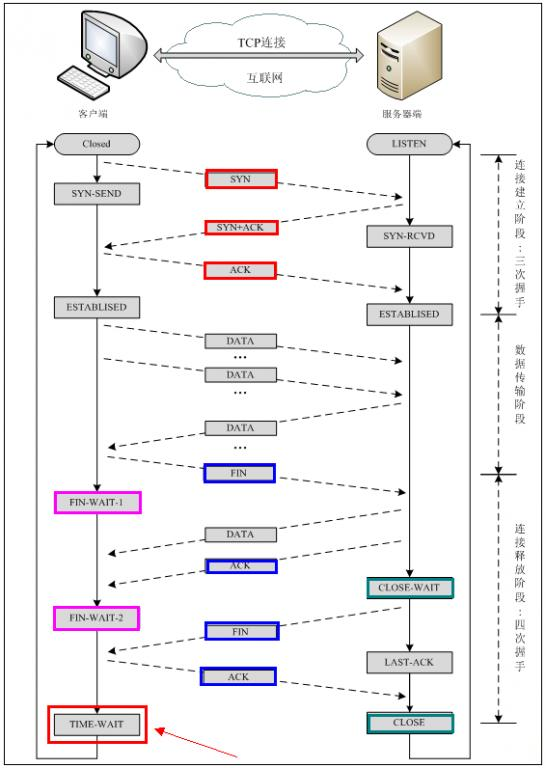
\includegraphics[scale = 0.5]{TCP-status.jpg}
				\caption{整个过程}
				\label{allstatus}
			\end{figure}
			
			\newpage		
			\begin{itemize}
				\item \verb|LISTEN|
				\item \verb|SYN_SENT|
				\item \verb|SYN_RCVD|
				\item \verb|ESTABLISHED|
				\item \verb|FIN_WAIT_1|:往一个已经接受FIN的套接字中写是允许的,接受到FIN仅仅代表对方不再发送数据了。
				\item \verb|CLOSE_WAIT|
				\item \verb|FIN_WAIT_2|
				\item \verb|LAST_ACK|
				\item \verb|TIME_WAIT|
				\item \verb|CLOSED|
				\item \verb|CLOSING|:双方同时关闭的情况
			\end{itemize}

		\newpage
		\subsection{3次握手:建立链接}
			首先Client端发送连接请求报文,Server段接受连接后回复ACK报文,并为这次连接分配资源。Client端接收到ACK报文后也向Server段发生ACK报文,并分配资源,这样TCP连接就建立了,如图\ref{3times}.
			
			\begin{figure}[ht]
				\centering
				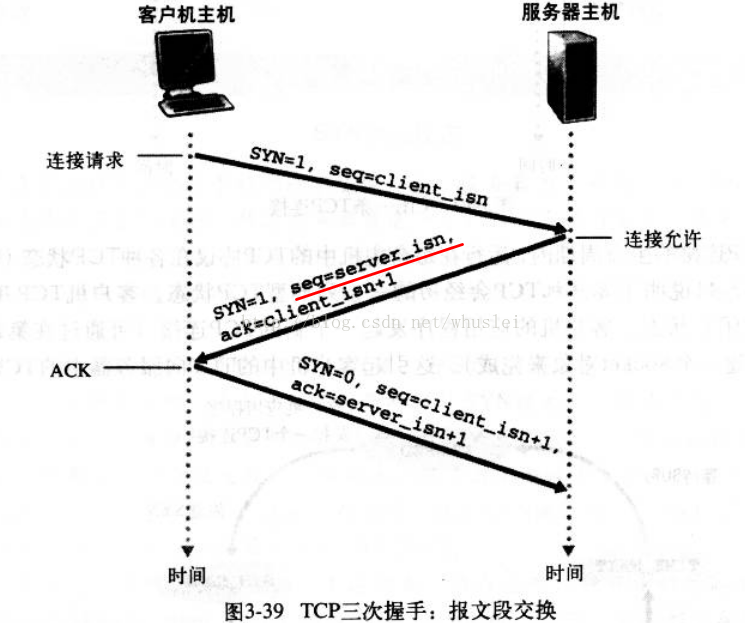
\includegraphics[scale = 0.5]{TCP-3times.png}
				\caption{3次握手}
				\label{3times}
			\end{figure}
			
			\begin{itemize}
				\item Client请求连接:\verb|SYN_SENT|
					
					客户端TCP首先给服务器端TCP发送一个\textbf{特殊的TCP数据段}。该数据段\textit{不包含应用层数据},并将头部中的\verb|SYN|\textbf{位设置为}\verb|1|,所以\textit{该数据段}被称为\textbf{SYN数据段}。另外,客户\textbf{选择一个初始序列号}\verb|SEQ|,设\verb|SEQ=x|并将这个编号\textbf{放到}初始的TCP \verb|SYN|\textbf{数据段的序列号字段中}。该数据段被封装到一个\verb|IP|数据报中,并发送给服务器。
				
				\item Server同意连接并发送确认代码:\verb|SYN_RCVD|
				
					一旦装有TCP \verb|SYN|数据段的IP数据报到达了服务器主机,服务器将从该数据报中\textbf{提取出}TCP \verb|SYN|数据段,给该连接\textbf{分配TCP缓冲区和变量},并给客户TCP\textbf{发送一个允许连接的数据段}。这个允许连接的数据段也\textbf{不包含任何应用层数据}。但是,它的头部中装载着3个重要信息。首先,\verb|SYN|被\textbf{设置为1};其次,TCP数据段头部的\textbf{确认字段被设置为}\verb|x+1|;最后,服务器\textbf{选择自己的初始顺序号},\verb|SEQ=y|,并将该值放到TCP数据段头部的序列号字段中。
					
				\item Client确认连接:\verb|ESTABLISHD|
				
					在接收到允许连接数据段之后,客户也会给连接分配缓冲区和变量。客户端主机还会给服务器发送另一个数据段,对服务器的允许连接数据段给出确认。
					
			\end{itemize}
			
		\newpage
		\subsection{4次握手:终止链接}
			断开连接简单的过程如下
			\begin{figure}[ht]
				\centering
				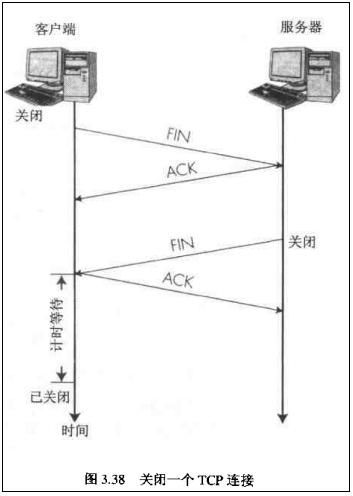
\includegraphics[scale = 0.7]{Tcp-close.png}
				\caption{Tcp 终止连接4次握手}
				\label{tcpClose}
			\end{figure}
			
			\begin{itemize}
				\item 一方A 关闭:\verb|FIN_WAIT_1|
				
					由进行数据通信的任意一方提出要求释放连接的请求报文段
					
				\item 另一方B 读取到\verb|FIN|消息后并发送确认代码:\verb|CLOSE_WAIT|
				
				\item 另一方B 当所有数据也都已经发送完毕后发送最后一个确认代码\verb|FIN|
				
					接收端收到此请求后,会发送确认报文段,同时当接收端的所有数据也都已经发送完毕后,接收端会向发送端发送一个带有其自己序号的报文段
					
				\item 一方A 未确认超过\verb|TIME_WAIT| 时间自动向服务器发送关闭确认
			\end{itemize}
		
			\textbf{中断连接端可以是Client端,也可以是Server端}
			
			假设Client端发起中断连接请求,也就是发送FIN报文。Server端接到\verb|FIN|报文后,意思是说"我Client端没有数据要发给你了",但是如果你还有数据没有发送完成,则不必急着关闭Socket,可以继续发送数据。所以你先发送\verb|ACK|,"告诉Client端,你的请求我收到了,但是我还没准备好,请继续你等我的消息"。这个时候Client端就进入\verb|FIN_WAIT|状态,继续等待Server端的\verb|FIN|报文。当Server端确定数据已发送完成,则向Client端发送\verb|FIN|报文,"告诉Client端,好了,我这边数据发完了,准备好关闭连接了"。Client端收到\verb|FIN|报文后,"就知道可以关闭连接了,但是他还是不相信网络,怕Server端不知道要关闭,所以发送\verb|ACK|后进入\verb|TIME_WAIT|状态,如果Server端没有收到\verb|ACK|则可以重传。“,Server端收到\verb|ACK|后,"就知道可以断开连接了"。Client端等待了\verb|2MSL|后依然没有收到回复,则证明Server端已正常关闭,那好,我Client端也可以关闭连接了。Ok,TCP连接就这样关闭了!
			
			\subsubsection{Client 经历的状态}
				整个过程Client端所经历的状态如下:
				\begin{figure}[ht]
					\centering
					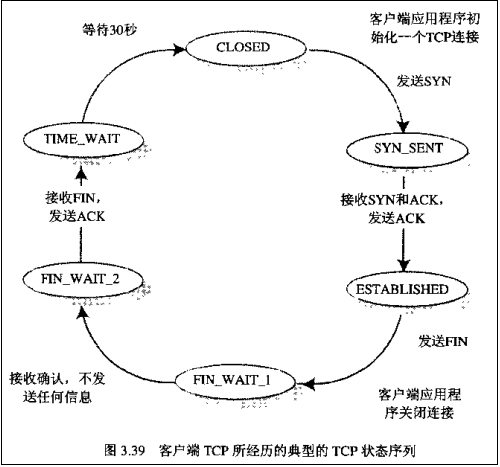
\includegraphics[scale = 0.7]{Client-status.png}
					\caption{Client 所有状态}
					\label{clientStatus}
				\end{figure}
			
			\subsubsection{Server 经历的状态}
			整个过程Server端所经历的状态如下:
			\begin{figure}[ht]
				\centering
				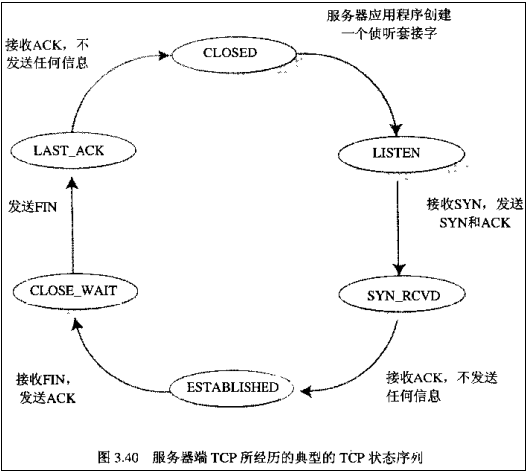
\includegraphics[scale = 0.7]{Server-status.png}
				\caption{Server 所有状态}
				\label{serverStatus}
			\end{figure}	
			
			\subsubsection{Notice}
				在\verb|TIME_WAIT|状态中,如果TCP client端最后一次发送的\verb|ACK|丢失了,它将重新发送。\verb|TIME_WAIT|状态中所需要的时间是依赖于实现方法的。典型的值为30秒、1分钟和2分钟。等待之后连接正式关闭,并且所有的资源(包括端口号)都被释放
				
				\subparagraph{为什么连接的时候是三次握手,关闭的时候却是四次握手?}
					答:因为当Server端收到Client端的\verb|SYN|连接请求报文后,可以直接发送\verb|SYN+ACK|报文。其中\verb|ACK|报文是用来应答的,\verb|SYN|报文是用来同步的。但是关闭连接时,当Server端收到FIN报文时,很可能并不会立即关闭\verb|SOCKET|,所以只能先回复一个\verb|ACK|报文,告诉Client端,"你发的\verb|FIN|报文我收到了"。只有等到我Server端所有的报文都发送完了,我才能发送\verb|FIN|报文,因此不能一起发送。故需要四步握手。
					
				\subparagraph{TIME\_WAIT 存在的理由}
					\begin{itemize}
						\item  虽然按道理,四个报文都发送完毕,我们可以直接进入\verb|CLOSE|状态了,但是\textbf{我们必须假象网络是不可靠的},有可以最后一个\verb|ACK|丢失。所以\verb|TIME_WAIT|状态就是用来\textbf{重发可能丢失的ACK报文},否则被动关闭端会出现RST错误。
						
						\item \verb|TIME_WAIT|第二个原因是为防止来自某个链接的老的重复分组在该链接已经终止后再现,从而被误解成属于同一链接的某个新的化身。为做到这一点,TCP将不给处于\verb|TIME_WAIT|状态的连接发起新的化身。
							
							而为什么是2MSL,有以下两方面因素
							\begin{itemize}
								\item 足以让某个被动关闭 方向上的分组最多存活MSL即被丢弃
								\item 主动关闭方向上的应答 最多存活MSL秒也被丢弃
							\end{itemize}
						
					\end{itemize}
	\section{套接字选项}
		\subsection{相关函数}
			\begin{itemize}
				\item \verb|int getsockopt(int sockfd, int level, int optname, void *optval, socklen_t *optlen);|
				\item \verb|int setsockopt(int sockfd, int level, int optname, void *optval, socklen_t *optlen);|
					\begin{enumerate}
						\item socketfd(套接字描述符)
						\item level(级别),如果想要在\textbf{套接字级别}上设置选项,就必须把level设置为\verb|SOL_SOCKET|
							\begin{itemize}
								\item \verb|SOL_SOCKET|: 基本套接口
								\item \verb|IPPROTO_IP|: IPv4套接口
								\item \verb|IPPROTO_IPV6|: IPv6套接口
								\item \verb|IPPROTO_TCP|: TCP套接口
							\end{itemize}
						\item optname(选项名): 选项名称
						\item optval(选项值): 是一个指向变量的指针 
						\item optlen(选项长度) :\verb|optval| 的大小
						
							\verb|->Typical Code|
							\begin{lstlisting}[frame=L]
	int nZero=0;
	setsockopt(socket, SOL_S0CKET, SO_SNDBUF, (char *)&nZero, sizeof(nZero));
							\end{lstlisting}
					\end{enumerate}
				\item \verb|int fcntl(int fd, int cmd, … /* arg */);|
					\begin{lstlisting}[frame=L]
	// 将描述符设置为 非阻塞
	int flags;
	flags = fcntl(fd, F_GETFL, 0);
	flags |= O_NONBLOCK;
	fcntl(fd, F_SETFL, flags);
	
	// 关闭非阻塞
	flags &= ~O_NONBLOCK;
	fcntl(fd, F_SETFL, flags);	
					\end{lstlisting}
				\item \verb|*ioctl()|
			\end{itemize}
		\subsection{低水位标记}
			分为接受低水位标记 和 发送低水位标记,目的在于:它允许应用进程 控制 在select返回可读或可写条件之前 有多少数据可读或有多少空间可用于写。
			
			\verb|-> Example:|如果我们知道除非至少存在64个字节的数据,否则我们的应用进程没有任何有效工作可做,那么可以把接受低水位标记设置为64,以防少于64个字节的数据准备好读时\verb|select|唤醒我们。
		\subsection{高水位标记}
			当你能够迅速从进程向进程发送消息时,你很快就会发现,\textbf{内存是宝贵的资源,并且很容易填满}。除非你理解这个问题,并采取预防措施,否则在进程中某处几秒钟的延迟,都可能变成撑爆一个服务器的积压。
			
			\subparagraph{问题}如果有一个\verb|进程A| 正发送消息给\verb|进程B|,而\verb|进程B| 突然变得非常繁忙(执行垃圾收集,CPU 过载,等等),那么\verb|进程A| 要发送的消息会发生什么情况呢?\textit{有些消息}会位于\verb|B| 的网络缓冲区,\textit{有些消息}会位于以太网线路本身,\textit{有些消息}会位于A 的网络缓冲区,\textbf{其余的}\textbf{会积聚在A 的内存中}。
			如果不采取一些预防措施,A 很容易就会耗尽内存并且崩溃。\textbf{这是消息代理的一个经典问题}。
		
			\subparagraph{解决办法}一个办法是将问题交给上游。\verb|A| 是从别的地方得到的消息,所以\textbf{可以告诉}该进程停下来,排队,这就是所谓的\textbf{流量控制}。这听起来不错,但如果你发送的是Twitter 的微博呢?你能告诉整个世界,在\verb|B| 采取行动时停止发微博吗?
			
			\textbf{流量控制}在某些情况下能够工作,而在有些情况下不能工作。\textbf{传输层也不能叫应用层“停止”},好比地铁系统不可以告诉一个大型企业,“请让你的员工继续工作半小时。我太忙了。”
			
			对于\textbf{消息传递},解决办法是\textbf{设置缓冲区的大小限制},然后,当我们到达这些限制时,采取一些明智的行动。\verb|在某些情况下|(不过不是一个地铁系统),答案是\textbf{丢弃消息}。\verb|在其他情况下|,最好的策略是\textbf{等待}。
			
			\verb|.MQ| 使用\textbf{高水位标记}(high-water mark,HWM)的概念\textbf{来定义其内部管道的容量}。每个从套接字出来或连入套接字的连接都有它自己用于发送和 或接收的管道和HWM,这取决于套接字类型。\verb|有些套接字|(PUB、PUSH)只有发送缓冲区,\verb|有些套接字|(SUB、PULL、REQ、REP)只有接收缓冲区,\verb|有些套接字|(DEALER、ROUTER、PAIR)同时具有发送缓冲区和接收缓冲区。
			
			在.MQ v2.x 版本中,HWM 默认是无限的。在.MQ v3.x 版本,它在默认情况下为1000,这是比较明智的设置。如果你还在使用.MQ v2.x 版本,你应该总是在你的套接字上设置HWM,无论是设置为1000 以匹配.MQ v3.x,还是设置为另一个考虑到你的消息大小的数字。
			
			\textbf{当你的套接字达到其HWM 时},根据不同的套接字类型,\textbf{这将阻塞或删除数据}。如果它们达到其HWM,PUB 和ROUTER 套接字\textbf{将丢弃数据},而其他类型的套接字\textbf{将阻塞}。通过inproc 传输时,发送者和接收者共享同一个缓冲区,所以真正的HWM 等于由两侧设置的HWM 的总和。
			
		\subsection{SO\_KEEPALIVE}			
		给一个TCP套接字设置保持存活选项后,如果\textbf{2小时内}在该套接字的任何一方向上都\textbf{没有数据交换},TCP就自动给对端发送一个保持存活探测分节。这是一个对端必须响应的tcp分节,它会导致以下三种情况之一:
			\begin{itemize}
				\item 对端\textbf{以}期望的\verb|ACK|\textbf{响应}。应用进程得不到通知(因为一切正常)。在又经过仍无动静的2小时后,\verb|TCP|将发出另一个探测分节。
				\item 对端\textbf{以}\verb|RST|\textbf{响应},它告知本端\verb|TCP|:对端已崩溃且已重新启动。该套接字的待处理错误被置为\verb|ECONNRESET|,套接字本身则被关闭。
				\item 对端对保持存活探测分节\textbf{没有}任何\textbf{响应}。
			\end{itemize}
			
			\textbf{如果}根本\textbf{没有}对TCP的探测分节的\textbf{响应},该套接字的\textbf{待处理错误就被置为}\verb|ETIMEOUT|,\textbf{套接字本身则被关闭}。\textbf{然而如果}该套接字收到一个\verb|ICMP错误|\textbf{作为}某个探测分节的\textbf{响应},那就\textbf{返回响应的错误},\textbf{套接字本身也被关闭}。
			
			本选项的\textit{功能是}\textbf{检测对端主机是否崩溃或变的不可达}(譬如拨号调制解调器连接掉线,电源发生故障等等)。\textbf{如果}\textit{对端进程崩溃},它的TCP将跨连接发送一个FIN,这可以通过调用select很容易的检测到。
			
			\textbf{本选项一般由服务器使用},不过客户也可以使用。服务器使用本选项时因为他们花大部分时间阻塞在等待穿越TCP连接的输入上,也就是说在等待客户的请求。然而如果客户主机连接掉线,电源掉电或者系统崩溃,服务器进程将永远不会知道,并将继续等待永远不会到达的输入。我们称这种情况为\textbf{半开连接}。\textbf{保持存活选项}\textit{将检测出这些半开连接并终止他们}。
			
			\begin{figure}[h]
				\centering
				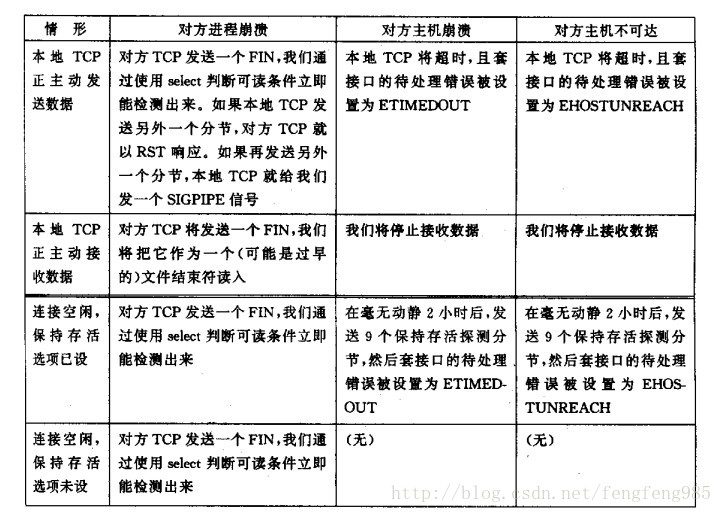
\includegraphics[scale = 0.9]{keepAlive.jpg}
				\caption{keepAlive}
			\end{figure}
			
			可以缩短TCP的保持存活定时器参数改为一个小的多的值,但是这些参数通常是按照内核而不是按照每个套接字维护的。
			
			KeepAlive,参数修改:\url{http://blog.csdn.net/callinglove/article/details/38380673}
			
			
		\subsection{SO\_LINGER}本选项\textbf{指定}\verb|close|函数对\textbf{面向连接的协议}(例如TCP和SCTP,但不是UDP)\textbf{如何操作}。默认操作是close立即返回,但是\textbf{如果有数据残留在套接字发送缓冲区中,系统将试着把这些数据发送给对端}。
			
			\verb|->|如果\textbf{选择此选项},\verb|close|或 \verb|shutdown|将\textbf{等到}所有套接字里排队的\textbf{消息成功发送}或到达延迟时间后\textbf{才会返回}。\textbf{否则,调用将立即返回}。
			
			\begin{lstlisting}[frame=L]
	struct linger {  
		int   l_onoff;      //  1 is on, 0 is off
		int   l_linger;     //  wait time
	};  
			\end{lstlisting}
			
			如果在发送数据的过程中(\verb|send()|没有完成,还有数据没发送)而调用了\verb|closesocket()|,以前我们一般采取的措施是"从容关闭"\verb|shutdown(s,SD_BOTH)|,但是数据是肯定丢失了,如何设置让程序满足具体应用的要求(即让没发完的数据发送出去后在关闭\verb|socket|)?
			\begin{lstlisting}[frame=L]	
	linger m_sLinger;
	m_sLinger.l_onoff=1;//在closesocket()调用,但是还有数据没发送完毕的时候容许延时关闭
	m_sLinger.l_linger=5;//容许逗留的时间为5秒
	
	setsockopt(s,SOL_SOCKET,SO_LINGER,(const char*)&m_sLinger,sizeof(linger));
			\end{lstlisting}
			
		\subsection{SO\_RCVBUF}
			每个套接字都有一个发送缓冲区和一个接收缓冲区。
			
			\textbf{接收缓冲区}被TCP,UDP和SCTCP\textit{用来保存接收到的数据},\textbf{直到}由应用进程读取。对于TCP来说,\textbf{套接字接收缓冲区可用空间的大小}\underline{限制了}TCP\textbf{通告对端的窗口大小}。TCP套接字\textbf{接收缓冲区不可以溢出},因为不允许对端发出超过本端所通告窗口大小的数据。\textbf{这就是TCP的流量控制},如果对端无视窗口大小而发出了超过窗口大小的数据,本端TCP将丢弃它们。\textbf{然而对于UDP来说},\textit{当接收到的数据报装不进套接字接收缓冲区时,该数据报就被丢弃}。回顾一下,UDP是没有流量控制的:较快的发送端可以很容易的淹没较慢的接收端,导致接收端的UDP丢弃数据报。
			
			这两个套接字选项允许我们改变着两个缓冲区的默认大小。对于不同的实现,默认值得大小可以有很大的差别。如果主机支持NFS,那么\textbf{UDP发送缓冲区的大小}经常\textbf{默认为9000字节左右}的一个值,而\textbf{UDP接收缓冲区}的大小则经常\textbf{默认为40000字节左右}的一个值。
			
			当设置TCP套接字接收缓冲区的大小时,\textbf{函数调用的顺序很重要}。这是因为\textbf{TCP的出口规模选项}是\textbf{在建立连接时}用\verb|SYN|分节与对端互换得到的。
			
			\textbf{对于客户},这意味着\verb|SO_RCVBUF|选项\textbf{必须在}调用\verb|connect|\textbf{之前设置};
			
			\textbf{对于服务器},这意味着该选项必须\textbf{在}调用\verb|listen|\textbf{之前给监听套接字设置}。给已连接套接字设置该选项对于可能存在的出口规模选项没有任何影响,因为\verb|accept|直到TCP的三路握手完成才会创建并返回已连接套接字。这就是必须给监听套接字设置本选项的原因。
			
		\subsection{SO\_SNDBUF}
			在\verb|send()|的时候,返回的是\textbf{实际发送出去}的字节(\textbf{同步})或\textbf{发送到socket缓冲区}的字节(\textbf{异步});
			
			系统默认的状态发送和接收一次为8688字节(约为8.5K);\textit{在实际的过程中发送数据和接收数据量比较大},\textbf{可以设置socket缓冲区},而\textbf{避免}了\verb|send(),recv()不断的循环收发|:
			
			\begin{lstlisting}[frame=L]
	// 接收缓冲区
	int nRecvBuf=32*1024;//设置为32K
	setsockopt(s,SOL_SOCKET,SO_RCVBUF,(const char*)&nRecvBuf,sizeof(int));
	//发送缓冲区
	int nSendBuf=32*1024;//设置为32K
	setsockopt(s,SOL_SOCKET,SO_SNDBUF,(const char*)&nSendBuf,sizeof(int));
		\end{lstlisting}
		
		\subsection{SO\_RCVLOWAT}
		\subsection{SO\_SNDLOWAT}
		\subsection{SO\_RCVTIMEO}
			这两个选项允许我们给套接字的接收和发送设置一个超时值。注意,访问他们的\verb|getsockopt|和\verb|setsockopt|函数的参数是指向\verb|timeval|结构的指针,与\verb|select|所用参数相同。这可让我们用秒数和微妙数来规定超时。我们通过设置其值为0s和0μs来禁止超时。默认情况下着两个超时都是禁止的。
			
			接收超时影响5个\textbf{输入函数}:\verb|read,readv,recv,recvfrom和recvmsg|。
			
			发送超时影响5个\textbf{输出函数}:\verb|write,writev,send,sendto和sendmsg|。
			
		\subsection{SO\_SNDTIMEO}
			在\verb|send(),recv()|过程中有时由于网络状况等原因,发收不能预期进行,而设置收发时限:
			\begin{lstlisting}[frame=L]
	int nNetTimeout=1000;//1秒
	//发送时限
	setsockopt(socket,SOL_S0CKET,SO_SNDTIMEO,(char *)&nNetTimeout,sizeof(int));
	//接收时限
	setsockopt(socket,SOL_S0CKET,SO_RCVTIMEO,(char *)&nNetTimeout,sizeof(int));
			\end{lstlisting}
			
		\subsection{SO\_REUSERADDR}
			关闭套接字后, 一般不会立即关闭而经历\verb|TIME_WAIT|的过程,后想立即重用该地址:
			\begin{lstlisting}[frame=L]
	BOOL bReuseaddr=TRUE;
	setsockopt(s,SOL_SOCKET ,SO_REUSEADDR,(const char*)&bReuseaddr,sizeof(BOOL));
			\end{lstlisting}
			
		\subsection{SO\_BROADCAST}
			本选项开启或禁止进程发送广播消息的能力。只有数据报套接字支持广播,并且还必须是在支持广播消息的网络上(例如以太网,令牌环网等)。我们不可能在点对点链路上进行广播,也不可能在基于连接的传输协议(例如TCP和SCTP)之上进行广播。
			
		\subsection{SO\_DEBUG}
			本选项仅由TCP支持。当给一个TCP套接字开启本选项时,内核将为TCP在该套接字发送和接受的所有分组保留详细跟踪信息。这些信息保存在内核的某个环形缓冲区中,并可使用trpt程序进行检查。
		
		\subsection{SO\_OOBINLINE}
			默认是禁止的,这样对于接受套接字来说,\textbf{该数据字节}\textit{不放入套接字接收缓冲区},而是\textbf{被放入该链接的一个独立的单字节带外缓冲区}。接受进程从单字节缓冲区读入数据的\textbf{唯一方法}是  使用\verb|MSG_OOB|标志调用 recv、recvfrom、recvmsg。
			
			当本选项开启时,带外数据将留在正常的输入队列中。这种情况,接受进程不能使用\verb|MSG_OOB|读入数据字节。	
			
		\subsection{TCP\_MAXSEG}	
			TCP 最大分节大小
		
		\subsection{TCP\_NODELAY}
			禁止Nagle 算法。
			
		\subparagraph{参考}\url{http://blog.sina.com.cn/s/blog_b4ef897e0102vrtt.html}
	
	\section{带外数据-Urgent标志}
		即使数据的流动会因为TCP的流量控制而停止,紧急通知却总是无障碍的发送到对端TCP。
	
		\url{http://blog.csdn.net/ordeder/article/details/43243425}
	\section{心搏函数-弥补keepAlive2小时等待时间}	
			
	\section{高级IO函数}
		\subsection{创建文件描述符系列}
			\subsubsection{pipe}
				pipe 函数可用于\textbf{创建一个单向管道},以 实现 \textbf{进程间通信}。
			
				\begin{itemize}
					\item 头文件 \verb|#include<unistd.h>|
					\item 函数原型:\verb|int pipe(int filedes[2]);|\verb|pipe()|会建立管道,并将文件描述符由参数\verb|filedes|数组返回
						\begin{enumerate}
							\item  \verb|filedes[0]|为管道里的读取端
							\item  \verb|filedes[1]|则为管道的写入端
						\end{enumerate}
				\end{itemize}
				
				\begin{lstlisting}
	#include <unistd.h>  
	#include <stdio.h>  
	
	int main( void )  
	{  
		int filedes[2];  
		char buf[80];  
		pid_t pid;  
		
		pipe( filedes );  
		pid=fork();          
		if (pid > 0)  
		{  
			printf( "This is in the father process,here write a string to the pipe.\n" );  
			char s[] = "Hello world , this is write by pipe.\n";  
			write( filedes[1], s, sizeof(s) );  
			close( filedes[0] );  
			close( filedes[1] );  
		}  
		else if(pid == 0)  
		{  
			printf( "This is in the child process,here read a string from the pipe.\n" );  
			read( filedes[0], buf, sizeof(buf) );  
			printf( "%s\n", buf );  
			close( filedes[0] );  
			close( filedes[1] );  
		}  
		
		waitpid( pid, NULL, 0 );  
		
		return 0;  
	}  
				\end{lstlisting}
			\subsubsection{socketpair}
				创建双向管道
				
				\begin{itemize}
					\item 函数原型:\verb|int socketpair(int d, int type, int protocol, int fd[2]);|   
						\begin{enumerate}
							\item 第1个参数\verb|d|,表示\textbf{协议族},只能为\verb|AF_LOCAL|或者\verb|AF_UNIX|;
							\item 第2个参数\verb|type|,表示\textbf{类型},只能为0。
							\item 第3个参数\verb|protocol|,表示\textbf{协议},可以是\verb|SOCK_STREAM|或者\verb|SOCK_DGRAM|。用\verb|SOCK_STREAM|建立的套接字对是管道流,与一般的管道相区别的是,套接字对建立的通道是双向的,即每一端都可以进行读写。
							\item 第4个参数\verb|fd|,用于\textbf{保存建立的套接字对}.
						\end{enumerate}
				\end{itemize}
				
				Demo: \url{http://blog.csdn.net/u012719256/article/details/52945310}
				
			\subsubsection{dup..复制}\verb|dup| 函数 创建 一个 新的 文件 描述 符, 该 新 文件 描述 符 和 原有 文件 描述 符 \verb|file_ descriptor| 指向 相同 的 文件、 管道 或者 网络 连接。 并且 \verb|dup| 返回 的 文件 描述 符 总是 取 系统 当前 可用 的 最小 整 数值。
			
				\verb|int dup( int oldfd ); |
				\subparagraph{执行dup 前}
				
					\begin{figure}[h]
						\centering
						\includegraphics*[scale = 0.8]{orgi.png}
						\caption{执行dup 前}
					\end{figure}
				
				\subparagraph{执行dup 后}
					\verb|Dup|函数总是\textbf{从数组第一个元素开始扫描},获取第一个可用的文件描述符(也就是没有关联实际文件的fd),这就是所谓:\textbf{dup总是使用最小的文件描述符}。理解了原理就简单了。
					
					\begin{figure}[h]
						\centering
						\includegraphics*[scale = 0.8]{after.png}
						\caption{执行dup 后}
					\end{figure}
					
				\subparagraph{例子}一般来说,初始化的时候,进程都拥有默认的三个文件描述符默认代表,标准输入,标准输出,标准错误。但是这不是硬性规定,你可以自己改呀!例如下面的代码:
					\begin{lstlisting}
	close(0);
	dup(fd[x]);/* 这是一个普通文件的文件描述符 */
					\end{lstlisting}	
			
				这之后,你会发现,0号文件描述符关联上了这个文件(0是最小的文件描述符,所以肯定会被dup选中!
				
				理解: \url{http://blog.csdn.net/shanshanpt/article/details/39049579}
				
			\subsubsection{dup2.. 重定向}
				类似于linux 下的\textbf{重定向命令},将某个输出重定向到某个文件,对于dup2, 相当于将targetfd 重定向 到oldfd。\verb|dup2|函数成功返回时,目标描述符(\verb|dup2|函数的第二个参数)将变成源描述符(\verb|dup2|函数的第一个参数)的复制品,换句话说,两个文件描述符现在都指向同一个文件,并且是函数第一个参数指向的文件。
				
				\verb|int dup2( int oldfd, int targetfd );|
				
				\subparagraph{*例子} 用dup 复制保存原文件描述符指向, 用dup2 重定向其到其他文件, 最后再还原。
					\begin{lstlisting}
	int main()  
	{  
		int sfd = dup(STDOUT_FILENO), testfd;  
		
		printf("sfd = [%d]\n", sfd);  
		
		testfd = open("./temp",O_CREAT | O_RDWR | O_APPEND);  
		if (-1 == testfd)  
		{  
			printf("open file error.\n");  
			exit(1);  
		}  
		
		/* 重定向 */  
		if (-1 == dup2(testfd,STDOUT_FILENO) ) {  
			printf("can't redirect fd error\n");  
			exit(1);  
		}  
		
		/* 此时向stdout写入应该输出到文件 */  
		write(STDOUT_FILENO,"file\n",5);  
		
		/* 恢复stdout */  
		if (-1 != dup2(sfd,STDOUT_FILENO) ) {  
			printf("recover fd ok \n");  
			
			/* 恢复后,写入stdout应该向屏幕输出 */  
			write(STDOUT_FILENO,"stdout\n",7);  
		}  
		
		printf("gogogogogogo!\n");  
		close(testfd);  
	}  
					\end{lstlisting}
				
		\subsection{读写数据系列}
			\subsubsection{readv/writev}
				\verb|readv| 函数 将 数据 从文 件 描述 符 读到 分散 的 内存 块 中, 即 分散 读; 
				
				\verb|writev| 函数 则 将 多块 分散 的 内存 数据 一并 写入 文件 描述 符 中, 即 集中 写。
				
			\subsubsection{sendfile}
				\verb|sendfile| 函数 在 两个 文件 描述 符 之间 直接 传递 数据(\textbf{完全在内核中操作}), 从而 避免 了 内核 缓冲区 和 用户 缓冲区 之间 的 数据 拷贝, 效率 很高, 这 被称为 零 拷贝。
			
			\subsubsection{mmap/munmpa}
				内存映射见IPC
				
			\subsubsection{splice}
				\verb|splice| 函数 用于 在 两个 文件 描述 符 之间 移动 数据, 也是 \textbf{零拷贝 操作}。
				
			\subsubsection{tee}
				\verb|tee| 函数 在 两个 管道 文件 描述 符 之间 复制 数据, 也是 零 拷贝 操作。 它不 消耗 数据, 因此 源 文件 描述 符 上 的 数据 仍然 可以 用于 后续 的 读 操作。
			
		\subsection{控制IO行为和属性系列}
			\subsubsection{fcntl}
	
	\section{IPC}
		\subsection{IPC 简介}
			
		\subsection{信号}
			\url{http://blog.csdn.net/ljianhui/article/details/10128731}
		\subsection{消息传递}
		
		\subsection{信号量}
			\subsubsection{信号量}
				\url{http://blog.csdn.net/ljianhui/article/details/10243617}
				\paragraph{简介}
					为了\textbf{防止}出现因\textbf{多个程序同时访问一个共享资源}而引发的一系列问题,我们需要一种方法,它可以通过生成并使用令牌来授权,在任一时刻只能有一个执行线程访问代码的临界区域。
					
					\textbf{临界区域}是指执行数据更新的代码需要独占式地执行。
					
					而信号量就可以提供这样的一种访问机制,让一个临界区同一时间只有一个线程在访问它,也就是说信号量是用来调协进程对共享资源的访问的。
					
					信号量是一个特殊的变量,程序对其访问都是原子操作,且只允许对它进行\textbf{等待(即P(信号变量))}和\textbf{发送(即V(信号变量))信息}操作。最简单的信号量是只能取0和1的变量,这也是信号量最常见的一种形式,叫做\textbf{二进制信号量}。而可以取多个正整数的信号量被称为\textbf{通用信号量}。
					
				\paragraph{工作原理}
					信号量只能进行两种操作-P与V 操作
						\begin{itemize}
							\item \verb|P(sem)|:如果\verb|sem|的值\textbf{大于零},就给它\textbf{减1};如果它的值\textbf{为零},就\textbf{挂起}该进程的执行
							\item \verb|V(sem)|:如果\textbf{有其他进程因等待}\verb|sem|而被挂起,就让它\textbf{恢复运行},如果\textbf{没有进程}因\textbf{等待}\verb|sem|而挂起,就给它\textbf{加1}
						\end{itemize}
				
				\paragraph{使用}
					\begin{itemize}
						\item \verb|int semget(key_t key, int num_sems, int sem_flags); |// 创建一个新信号量或取得一个已有信号量
							\begin{enumerate}
								\item \verb|key|是整数值(唯一非零),不相关的进程可以通过它访问一个信号量,它\textbf{代表}程序可能要使用的\textbf{某个资源}
								\item \verb|num_sems|指定\textbf{需要的信号量数目},它的值几乎总是1
								\item \verb|sem_flags|是一组标志,当想要当信号量不存在时创建一个新的信号量,可以和值\verb|IPC_CREAT|做按位或操作。设置了\verb|IPC_CREAT|标志后,即使给出的键是一个已有信号量的键,也不会产生错误。而\verb|IPC_CREAT||\verb|IPC_EXCL|则可以创建一个新的,唯一的信号量,如果信号量已存在,返回一个错误
							\end{enumerate}
						\item \verb|int semop(int sem_id, struct sembuf *sem_opa, size_t num_sem_ops);|  // 改变信号量的值
							\begin{enumerate}
								\item \verb|sem_id|是由\verb|semget|返回的\textbf{信号量标识符}
								\item \verb|sembuf|结构代表了某种操作
									\begin{lstlisting}[frame=L,xleftmargin=.05\textwidth]
	struct sembuf{  
		/*
			除非使用一组信号量,否则它为0 
		*/
		short sem_num; 
		
		/*
			信号量在一次操作中需要改变的数据,通常是两个数
			一个是-1,即P(等待)操作
			一个是+1,即V(发送信号)操作
		*/
		short sem_op;
		
		/*
			通常为SEM_UNDO,使操作系统跟踪信号
			并在进程没有释放该信号量而终止时,操作系统释放信号量
		*/ 
		short sem_flg;
	};  
									\end{lstlisting}
							\end{enumerate}
						\item \verb|int semctl(int sem_id, int sem_num, int command, ...);|  // 直接控制信号量信息(删除,传值)
					\end{itemize}
			
			\subsubsection{与互斥锁的区别}
				\subparagraph{信号量}
					信号量是一个特殊的变量,程序对其访问都是原子操作,且只允许对它进行等待(即P(信号变量))和发送(即V(信号变量))信息操作。我们通常通过信号来解决多个进程对同一资源的访问竞争的问题,使在任一时刻只能有一个执行线程访问代码的临界区域,也可以说它是协调进程间的对同一资源的访问权,也就是\textbf{用于同步进程的}。
			
		\subsection{共享内存}
			\subsubsection{虚拟内存}
				程序代码和数据必须驻留在内存中才能得以运行,然而系统内存数量很有限,往往不能容纳一个完整程序的所有代码和数据,更何况在多任务系统中,可能需要同时打开子处理程序,画图程序,浏览器等很多任务,想让内存驻留所有这些程序显然不太可能。\textbf{因此首先能想到的就是将程序分割成小份,只让当前系统运行它所有需要的那部分留在内存,其它部分都留在硬盘。}当系统处理完当前任务片段后,再从外存中调入下一个待运行的任务片段。的确,老式系统就是这样处理大任务的,而且这个工作是由程序员自行完成。但是随着程序语言越来越高级,程序员对系统体系的依赖程度降低了,很少有程序员能非常清楚的驾驭系统体系,因此放手让程序员负责将程序片段化和按需调入轻则降低效率,重则使得机器崩溃;再一个原因是随着程序越来越丰富,程序的行为几乎无法准确预测,程序员自己都很难判断下一步需要载入哪段程序。因此很难再靠预见性来静态分配固定大小的内存,然后再机械地轮换程序片进入内存执行。\textbf{系统必须采取一种能按需分配而不需要程序员干预的新技术}。
				
				\textbf{虚拟内存}(之所以称为虚拟内存,是和系统中的逻辑内存和物理内存相对而言的,\textbf{逻辑内存}是站在进程角度看到的内存,因此是程序员关心的内容。而\textbf{物理内存}是站在处理器角度看到的内存,由操作系统负责管理。
				
				\textbf{虚拟内存}可以说是映射到这两种不同视角内存的一个技术手段。)技术就是一种由操作系统接管的按需动态内存分配的方法,它允许程序不知不觉中使用大于实际物理空间大小的存储空间(其实是将程序需要的存储空间以页的形式分散存储在物理内存和磁盘上),所以说虚拟内存彻底解放了程序员,从此程序员不用过分关心程序的大小和载入,可以自由编写程序了,繁琐的事情都交给操作系统去做吧。

				\textbf{虚拟内存}是将系统硬盘空间和系统实际内存联合在一起供进程使用,给进程提供了一个比内存大得多的虚拟空间。\textbf{在程序运行时},只要把虚拟地址空间的一小部分映射到内存,其余都存储在硬盘上(也就是说程序虚拟空间就等于实际物理内存加部分硬盘空间)。\textbf{当被访问的虚拟地址不在内存时,}则说明该地址未被映射到内存,而是被存贮在硬盘中,因此需要的虚拟存储地址随即被调入到内存;同时\textbf{当系统内存紧张时,}也可以把当前不用的虚拟存储空间换出到硬盘,来腾出物理内存空间。系统如此周而复始地运转——换入、换出,而用户几乎无法查觉,这都是拜虚拟内存机制所赐。
			\subsubsection{mmap 系列}
				\verb|mmap|函数用来将文件映射进内存。需要指出的是这里的内存指的是\textbf{虚拟内存}。
				
				\verb|mmap|函数可以将一个文件的内容映射到内存,这样就可以直接对该内存进行操作,从而\verb|省去IO|操作。
				
				\verb|void *mmap(void *start, size_t length, int prot, int flags, int fd, off_t offset);|
				
				\begin{enumerate}
					\item \verb|start|:映射区的开始地址 (一般设置为NULL,让系统决定位置)
					\item \verb|length|:映射区的长度
					\item \verb|prot|:期望的内存保护标志,不能与文件的打开模式冲突。
						\begin{enumerate}
							\item \verb|PROT_EXEC| :页内容可以被执行
							\item \verb|PROT_READ| :页内容可以被读取
							\item \verb|PROT_WRITE |:页可以被写入
							\item \verb|PROT_NONE| :页不可访问
						\end{enumerate}
					\item \verb|flags|:指定映射对象的类型,映射选项和映射页是否可以共享。
						\begin{enumerate}
							\item \verb|MAP_SHARED| 与其它所有映射这个对象的进程共享映射空间。
							\item \verb|MAP_PRIVATE| 建立一个写入时拷贝的私有映射。
							\item \verb|MAP_ANONYMOUS| 匿名映射,映射区不与任何文件关联
						\end{enumerate}
					\item \verb|fd|:有效的文件描述词。如果\verb|MAP_ANONYMOUS|被设定,为了兼容问题,其值应为\verb|-1|
					\item \verb|offset|: 被映射对象内容的起点
				\end{enumerate}
		
				\verb|int munmap( void * addr, size_t len ); |
				
				该调用在进程地址空间中解除一个映射关系,addr是调用mmap()时返回的地址,len是映射区的大小;
				\subparagraph{例子}\verb|->|
				\begin{lstlisting}
	int main(int argc,char *argv[]){
		int fd,len;
		char *ptr;
		if(argc<2){
			printf("please enter a file\n");    
			return 0;
		}   
		if((fd=open(argv[1],O_RDWR))<0){
			perror("open file error");
			return -1; 
		}   
		len=lseek(fd,0,SEEK_END);   
		
		ptr=mmap(NULL,len,PROT_READ|PROT_WRITE,MAP_SHARED,fd,0);//读写得和open函数的标志相一致,否则会报错
		
		if(ptr==MAP_FAILED){
			perror("mmap error");
			close(fd);
			return -1; 
		}   
		close(fd);//关闭文件也ok
		printf("length is %d\n",strlen(ptr));
		printf("the %s content is:\n%s\n",argv[1],ptr);
		ptr[0]='c';//修改其中的一个内容
		printf("the %s content is:\n%s\n",argv[1],ptr);
		
		munmap(ptr,len);//将改变的文件写入内存
		
		return 0;
	}
				\end{lstlisting}
		
		\subsubsection{shmget 系列}
			共享内存并未提供同步机制,也就是说,在第一个进程结束对共享内存的写操作之前,并无自动机制可以阻止第二个进程开始对它进行读取。所以我们通常需要用其他的机制来同步对共享内存的访问
			
			\begin{itemize}
				\item \verb|int shmget(key_t key, size_t size, int shmflg);| 创建共享内存函数
				\item \verb|void *shmat(int shmid, const void *shmaddr, int shmflg);| Map 共享内存区
				\item \verb|int shmdt(const void *shmaddr);| unMap
				\item \verb|int shmctl(int shmid, int cmd,struct shmid_ds* buf);|删除共享内存  或管理
			\end{itemize}
			
			\subparagraph{例子}\verb|->|
				\url{https://github.com/ctzhenghua/C-NetworkPractice-Code/blob/Dev/IPCs/SharedMemory/shmRead.cc}
			
	\section{阻塞与非阻塞、同步与异步}
		\subsection{同步/异步主要针对C端}
			\begin{itemize}
				\item \textbf{同步}:所谓同步,就是在c端发出一个功能调用时,在没有得到结果之前,该调用就不返回。也就是必须一件一件事做,等前一件做完了才能做下一件事
				
				\textit{例如普通B/S模式(同步):提交请求->等待服务器处理->处理完毕返回 这个期间客户端浏览器不能干任何事}
				\item \textbf{异步}:  异步的概念和同步相对。当c端一个异步过程调用发出后,调用者不能立刻得到结果。实际处理这个调用的部件在完成后,通过状态、通知和回调来通知调用者
				
				\textit{例如 ajax请求(异步): 请求通过事件触发->服务器处理(这是浏览器仍然可以作其他事情)->处理完毕}
			\end{itemize}
		
		\subsection{阻塞/非阻塞主要针对S端}
			\begin{itemize}
				\item \textbf{阻塞}:阻塞调用是指调用结果返回之前,当前线程会被挂起(线程进入非可执行状态,在这个状态下,cpu不会给线程分配时间片,即线程暂停运行)。函数只有在得到结果之后才会返回。
				
				有人也许会把阻塞调用和同步调用等同起来,实际上他是不同的。对于同步调用来说,很多时候当前线程还是激活的,只是从逻辑上当前函数没有返回而已。 例如,我们在socket中调用recv函数,如果缓冲区中没有数据,这个函数就会一直等待,直到有数据才返回。而此时,当前线程还会继续处理各种各样的消息。
				
				\textit{快递的例子:比如到你某个时候到A楼一层(假如是内核缓冲区)取快递,但是你不知道快递什么时候过来,你又不能干别的事,只能死等着。但你可以睡觉(进程处于休眠状态),因为你知道快递把货送来时一定会给你打个电话(假定一定能叫醒你)。}
				\item \textbf{非阻塞}:非阻塞和阻塞的概念相对应,指在不能立刻得到结果之前,该函数不会阻塞当前线程,而会立刻返回。
				
				\textit{还是等快递的例子:如果用忙轮询的方法,每隔5分钟到A楼一层(内核缓冲区)去看快递来了没有。如果没来,立即返回。而快递来了,就放在A楼一层,等你去取。}
			\end{itemize}
		\subsection{Linux 下的5种I/O 模型}
			\subsubsection{阻塞I/O: Blocking I/O}进程会一直阻塞,直到数据拷贝完成
			
			应用程序调用一个IO函数,导致应用程序阻塞,等待数据准备好。 如果数据没有准备好,一直等待….数据准备好了,从内核拷贝到用户空间,IO函数返回成功指示。
			
			我们 第一次接触到的网络编程都是从 listen()、send()、recv()等接口开始的。使用这些接口可以很方便的构建服务器 /客户机的模型。
			
			\subparagraph{阻塞I/O模型图}:在调用recv()/recvfrom()函数时,发生在内核中等待数据和复制数据的过程。
			\begin{figure}[h]
				\centering
				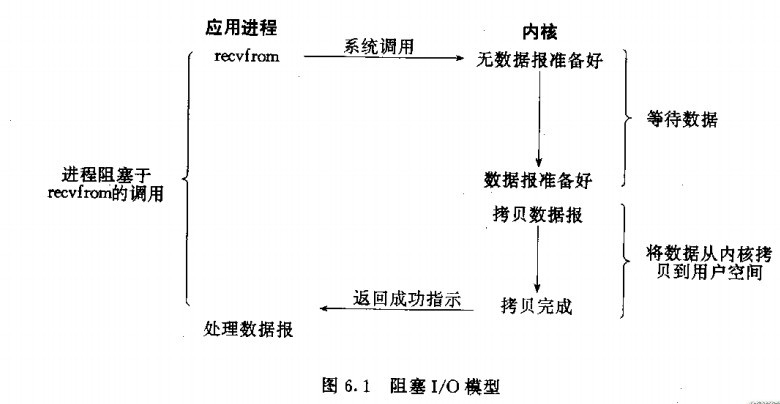
\includegraphics[scale = 0.8]{BlockingIO.jpg}
			\end{figure}
			
			当调用recv()函数时,系统首先查是否有准备好的数据。如果数据没有准备好,那么系统就处于等待状态。当数据准备好后,将数据从系统缓冲区复制到用户空间,然后该函数返回。在套接应用程序中,当调用recv()函数时,未必用户空间就已经存在数据,那么此时recv()函数就会处于等待状态。
			
			当使用socket()函数和WSASocket()函数创建套接字时,默认的套接字都是阻塞的。这意味着当调用Windows Sockets API不能立即完成时,线程处于等待状态,直到操作完成。
			
			并不是所有Windows Sockets API以阻塞套接字为参数调用都会发生阻塞。例如,以阻塞模式的套接字为参数调用bind()、listen()函数时,函数会立即返回。将可能阻塞套接字的Windows Sockets API调用分为以下四种:
			\begin{enumerate}[itemindent = 1em]
				\item 输入操作: recv()、recvfrom()、WSARecv()和WSARecvfrom()函数。以阻塞套接字为参数调用该函数接收数据。如果此时套接字缓冲区内没有数据可读,则调用线程在数据到来前一直睡眠
				\item 输出操作: send()、sendto()、WSASend()和WSASendto()函数。以阻塞套接字为参数调用该函数发送数据。如果套接字缓冲区没有可用空间,线程会一直睡眠,直到有空间
				\item 接受连接:accept()和WSAAcept()函数。以阻塞套接字为参数调用该函数,等待接受对方的连接请求。如果此时没有连接请求,线程就会进入睡眠状态
				\item 外出连接:connect()和WSAConnect()函数。对于TCP连接,客户端以阻塞套接字为参数,调用该函数向服务器发起连接。该函数在收到服务器的应答前,不会返回。这意味着TCP连接总会等待至少到服务器的一次往返时间
			\end{enumerate}
			
			使用阻塞模式的套接字,开发网络程序比较简单,容易实现。当希望能够立即发送和接收数据,且处理的套接字数量比较少的情况下,使用阻塞模式来开发网络程序比较合适。
			
			阻塞模式套接字的不足表现为,在大量建立好的套接字线程之间进行通信时比较困难。当使用“生产者-消费者”模型开发网络程序时,为每个套接字都分别分配一个读线程、一个处理数据线程和一个用于同步的事件,那么这样无疑加大系统的开销。其最大的缺点是当希望同时处理大量套接字时,将无从下手,其扩展性很差.
			
			阻塞模式给网络编程带来了一个很大的问题,如在调用 send()的同时,线程将被阻塞,在此期间,线程将无法执行任何运算或响应任何的网络请求。这给多客户机、多业务逻辑的网络编程带来了挑战。这时,我们可能会选择多线程的方式来解决这个问题。
			
			应对多客户机的网络应用,最简单的解决方式是在服务器端使用多线程(或多进程)。多线程(或多进程)的目的是让每个连接都拥有独立的线程(或进程),这样任何一个连接的阻塞都不会影响其他的连接。
			
			具体使用多进程还是多线程,并没有一个特定的模式。传统意义上,进程的开销要远远大于线程,所以,如果需要同时为较多的客户机提供服务,则不推荐使用多进程;如果单个服务执行体需要消耗较多的 CPU 资源,譬如需要进行大规模或长时间的数据运算或文件访问,则进程较为安全。通常,使用 pthread\_create () 创建新线程,fork() 创建新进程。
			
			多线程/进程服务器同时为多个客户机提供应答服务。模型如下:
			\begin{figure}[h]
				\centering
				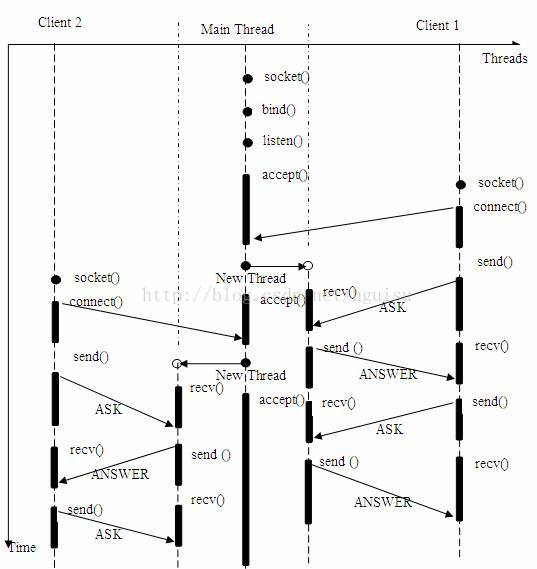
\includegraphics[scale = 0.8]{MultiThread.jpg}
			\end{figure}
			
			主线程持续等待客户端的连接请求,如果有连接,则创建新线程,并在新线程中提供为前例同样的问答服务。
			
			上述多线程的服务器模型似乎完美的解决了为多个客户机提供问答服务的要求,但其实并不尽然。如果要同时响应成百上千路的连接请求,则无论多线程还是多进程都会严重占据系统资源,降低系统对外界响应效率,而线程与进程本身也更容易进入假死状态。
			
			由此可能会考虑使用“线程池”或“连接池”。“线程池”旨在减少创建和销毁线程的频率,其维持一定合理数量的线程,并让空闲的线程重新承担新的执行任务。“连接池”维持连接的缓存池,尽量重用已有的连接、减少创建和关闭连接的频率。这两种技术都可以很好的降低系统开销,都被广泛应用很多大型系统,如apache,MySQL数据库等。
			
			但是,“线程池”和“连接池”技术也只是在一定程度上缓解了频繁调用 IO 接口带来的资源占用。而且,所谓“池”始终有其上限,当请求大大超过上限时,“池”构成的系统对外界的响应并不比没有池的时候效果好多少。所以使用“池”必须考虑其面临的响应规模,并根据响应规模调整“池”的大小。
			
			对应上例中的所面临的可能同时出现的上千甚至上万次的客户端请求,“线程池”或“连接池”或许可以缓解部分压力,但是不能解决所有问题。
			
			\subsubsection{非阻塞I/O: nonBlocking I/O}
			非阻塞IO通过进程反复调用IO函数(多次系统调用,并马上返回);在数据拷贝的过程中,进程是阻塞的
			
			我们把一个SOCKET接口设置为非阻塞就是告诉内核,当所请求的I/O操作无法完成时,不要将进程睡眠,而是返回一个错误。这样我们的I/O操作函数将不断的测试数据是否已经准备好,如果没有准备好,继续测试,直到数据准备好为止。在这个不断测试的过程中,会大量的占用CPU的时间。
			
			把SOCKET设置为非阻塞模式,即通知系统内核:在调用Windows Sockets API时,不要让线程睡眠,而应该让函数立即返回。在返回时,该函数返回一个错误代码。图所示,一个非阻塞模式套接字多次调用\verb|recv()|函数的过程。前三次调用\verb|recv()|函数时,内核数据还没有准备好。因此,该函数立即返回WSAEWOULDBLOCK错误代码。第四次调用\verb|recv()|函数时,数据已经准备好,被复制到应用程序的缓冲区中,\verb|recv()|函数返回成功指示,应用程序开始处理数据。
			
			\begin{figure}[h]
				\centering
				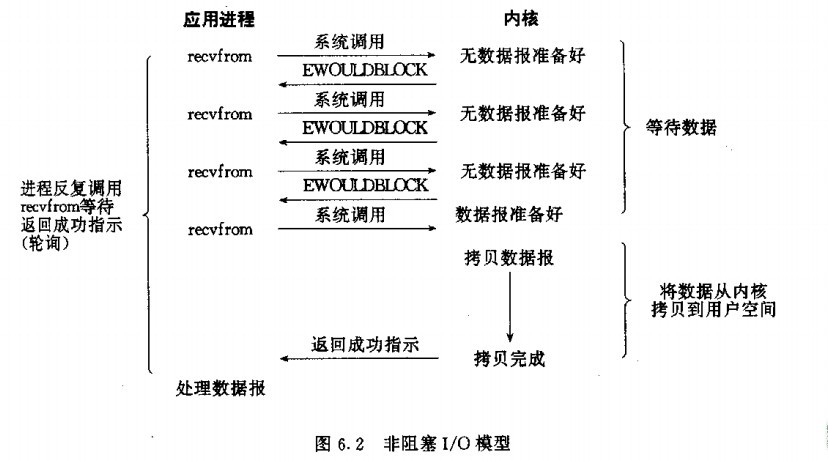
\includegraphics[scale = 0.8]{nonBlockingIO.jpg}
			\end{figure}
			
			当使用socket()函数和WSASocket()函数创建套接字时,默认都是阻塞的。在创建套接字之后,通过调用ioctlsocket()函数,将该套接字设置为非阻塞模式。Linux下的函数是:fcntl().
			套接字设置为非阻塞模式后,在调用Windows Sockets API函数时,调用函数会立即返回。大多数情况下,这些函数调用都会调用“失败”,并返回WSAEWOULDBLOCK错误代码。说明请求的操作在调用期间内没有时间完成。通常,应用程序需要重复调用该函数,直到获得成功返回代码。
			
			需要说明的是并非所有的Windows Sockets API在非阻塞模式下调用,都会返回WSAEWOULDBLOCK错误。例如,以非阻塞模式的套接字为参数调用bind()函数时,就不会返回该错误代码。当然,在调用WSAStartup()函数时更不会返回该错误代码,因为该函数是应用程序第一调用的函数,当然不会返回这样的错误代码。
			
			要将套接字设置为非阻塞模式,除了使用ioctlsocket()函数之外,还可以使用WSAAsyncselect()和WSAEventselect()函数。当调用该函数时,套接字会自动地设置为非阻塞方式。
			
			
			由于使用非阻塞套接字在调用函数时,会经常返回WSAEWOULDBLOCK错误。所以在任何时候,都应仔细检查返回代码并作好对“失败”的准备。应用程序连续不断地调用这个函数,直到它返回成功指示为止。上面的程序清单中,在While循环体内不断地调用\verb|recv()|函数,以读入1024个字节的数据。这种做法很浪费系统资源。
			
			要完成这样的操作,有人使用\verb|MSG_PEEK|标志调用\verb|recv()|函数查看缓冲区中是否有数据可读。同样,这种方法也不好。因为该做法对系统造成的开销是很大的,并且应用程序至少要调用\verb|recv()|函数两次,才能实际地读入数据。较好的做法是,使用套接字的“I/O模型”来判断非阻塞套接字是否可读可写。
			
			非阻塞模式套接字与阻塞模式套接字相比,不容易使用。使用非阻塞模式套接字,需要编写更多的代码,以便在每个Windows Sockets API函数调用中,对收到的WSAEWOULDBLOCK错误进行处理。因此,非阻塞套接字便显得有些难于使用。
			
			但是,非阻塞套接字在控制建立的多个连接,在数据的收发量不均,时间不定时,明显具有优势。这种套接字在使用上存在一定难度,但只要排除了这些困难,它在功能上还是非常强大的。通常情况下,可考虑使用套接字的“I/O模型”,它有助于应用程序通过异步方式,同时对一个或多个套接字的通信加以管理。
			
			\subsubsection{I/O复用: I/O multiplexing}
			主要是\verb|select|和\verb|epoll|;对一个IO端口,两次调用,两次返回,比阻塞IO并没有什么优越性;关键是能实现同时对多个IO端口进行监听
			
			\textbf{I/O复用模型}会用到\verb|select、poll、epoll|函数,这几个函数也会使进程阻塞,但是和\verb|阻塞I/O|所不同的的,这两个函数可以同时阻塞多个I/O操作。而且可以同时对多个读操作,多个写操作的I/O函数进行检测,直到有数据可读或可写时,才真正调用I/O操作函数。
			
			\begin{figure}[h]
				\centering
				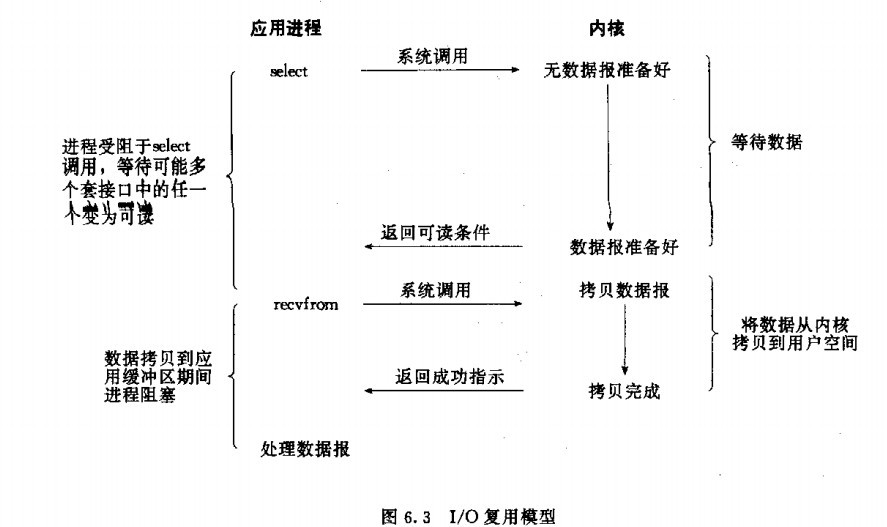
\includegraphics[scale = 0.8]{IOMultiplexing.jpg}
			\end{figure}
			\subsubsection{信号驱动I/O:SIGIO}
			
			\subsubsection{异步I/O:asynchronous I/O}只有这一种才是异步IO。数据拷贝的时候进程无需阻塞
			
			当一个异步过程调用发出后,调用者不能立刻得到结果。实际处理这个调用的部件在完成后,通过状态、通知和回调来通知调用者的输入输出操作
			
			\begin{figure}[h]
				\centering
				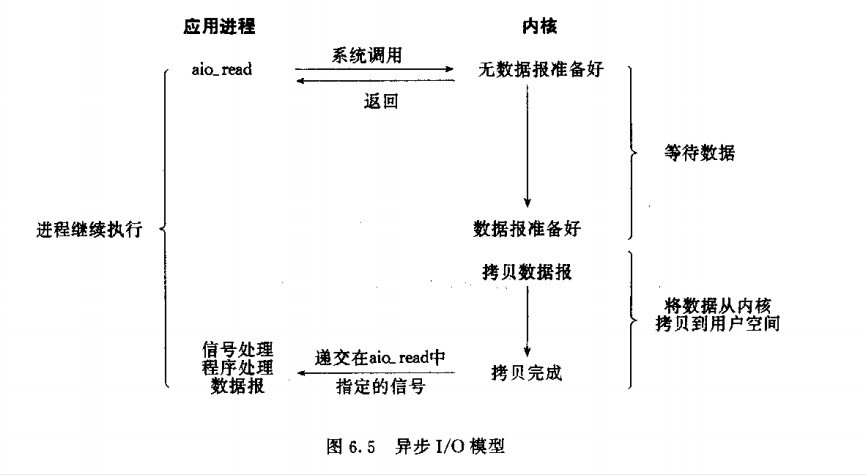
\includegraphics[scale = 0.8]{asyIO.jpg}
			\end{figure}
			
			同步IO引起进程阻塞,直至IO操作完成。
			
			异步IO不会引起进程阻塞。
			
			IO复用是先通过select调用阻塞
		\subsection{参考}\url{http://blog.csdn.net/hguisu/article/details/7453390}
	\section{Select 模型:管理多个IO}
		当一个服务器在处理多个客户时,它绝对不能阻塞于只与单个客户相关的某个函数调用,否则可能导致服务器挂起,拒绝为所有用户提供服务,所以是不是可以考虑半同步半异步的模式 或者 池的概念。
		\subsection{相关函数}
			\begin{itemize}
				\item \verb|int select(int nfds|[\textbf{最大套接字+1}]\verb|,fd_set *readfds|[\textbf{可读事件套接字集合-输入输出}]\verb|,fd_set *writefds|[\textbf{可写事件套接字集合-输入输出}]\verb|,fd_set *exceptfds|[\textbf{异常事件套接字集合-输入输出}], \verb|struct timeval* timeout);|
					
					\begin{itemize}
						\item null: 永远等待下去,仅在有一个描述符准备好I/O 才返回
						\item 0:	根本不等待,检查描述符后立即返回,这称为轮询方式
						\item timeval 结构: 等待结构中固定时间。
					\end{itemize}
					
				\textbf{用select 管理多个IO,一旦其中一个或多个IO检测到我们所感兴趣的事件,就函数返回检测到的事件个数和那些发生事件的IO标识符},然后我们遍历这些事件,分别处理
				
					\begin{itemize}
						\item 调用\verb|select|函数时\verb|fd_set|为值。
						\item 返回时的\verb|fd_set|为结果,即哪些描述符就绪了。
						\item 在\verb|fd_set| 中,任何与 \textbf{未就绪描述符}\textit{对应的}位, 在返回时均清为0。
					\end{itemize}
					
				\verb|-> Notice :|所以,\textbf{每次重新调用}\verb|select|函数时,我们\textbf{都得再次把所有关心的描述符}的位均置1. 
				
					\begin{itemize}
						\item 该函数的返回值表示 所有描述符集的已就绪的总位数
						\item 如果是定时器到时并且没有就绪的描述符,返回0
						\item 出错,返回-1
					\end{itemize}
				\item \verb|void FD_ZERO(fd_set *set)|:\textbf{将集合清空}
				\item \verb|void FD_SET(int fd,fd_set *set)|:\textbf{将fd 添加到集合set中}
				\item \verb|void FD_CLR(int fd,fd_set *set)|:\textbf{将fd 从集合set 中移除}
				\item \verb|int FD_ISSET(int fd,fd_set *set)|:\textbf{判断fd 是否在set中}
				\item \textbf{命令行: ulimit -n 最大并发数}:用该命令可以调整最大的并发个数
			\end{itemize}
			\paragraph{可读事件发生条件}
				\begin{itemize}
					\item 套接口\textbf{缓冲区有数据可读}:该套接字的\textbf{接收缓冲区中的数据字节数}\textit{大于等于}套接字\textbf{接受缓冲区低水位标记}的当前大小。
					
						可以使用\verb|SO_RCVLOWAT| 选项设置该套接字的低水位标记。对于\verb|TCP与UDP|默认为1.
					\item 连接的读一半关闭,即\textbf{接受到FIN段},读操作将返回0
					\item 如果是监听套接口,且已完成连接队列不为空时
					\item 套接口上发生了一个错误待处理:对这样的套接字的读操作将不阻塞并返回-1,同时把\verb|errno|设置为确切的错误条件。
					
					这些待处理错误可以通过\verb|getsockopt|指定\verb|SO_ERROR|选项来获取并清除。
				\end{itemize}
			\paragraph{可写事件发生条件}
				\begin{itemize}
					\item 套接口\textbf{发送缓冲区的可用数据字节数}\textit{大于等于}套接字\textbf{发送缓冲区的低水位标记}的当前大小。
					
						可以使用\verb|SO_SNDLOWAT| 来设置套接字的低水位标记,对于\verb|TCP与UDP|默认为\verb|2048|
					\item 连接的写一半关闭。即收到\verb|RST|段之后,再次调用\verb|write |操作\verb|->|产生\verb|SIGPIPE|信号
					\item 使用非阻塞式的\verb|connect| 的套接字已建立连接,或者\verb|connect| 已经以失败告终。
					
					\item 套接口上发生一个错误待处理,对这样的套接字的写操作将不阻塞并返回-1,同时把\verb|errno|设置为确切的错误条件。
					
					错误可以通过\verb|getsockopt|指定\verb|SO_ERROR|选项来获取并清除。
					
					\verb|-> Notice: |当套接字\textbf{发生错误时},它将由\verb|select|标记为\textbf{即可读又可写}。
				\end{itemize}
			\paragraph{异常事件发生条件}
				\begin{itemize}
					\item 套接口存在带外数据,\verb|urgent 位|为1.
				\end{itemize}
			
			\paragraph{最大处理描述符值}
				对于select 函数,所能处理的最大客户数目的限制是以下\textbf{两个值}中的较小者
					\begin{itemize}
						\item \verb|FD_SETSIZE|
						\item \verb|内核允许进程打开的最大描述符的值|
					\end{itemize}	
					
				是描述符fd的值而不是个数:\url{http://blog.csdn.net/adam040606/article/details/46833617}
				
				\verb|->Notice :|但是限制了最大值那么就限制了最大的个数。
		\subsection{使用select实现回射服务程序}
			\subsubsection{Client}
				\begin{lstlisting}
// Using Select to Implemet IO
	
	... sock stuff
	
	fd_set rset;
	FD_ZERO(&rset);
	
	int nready;
	int maxfd;
	int fd_stdin = fileno(stdin);
	maxfd = max(sock,fd_stdin);
	
	while(1)
	{
		FD_SET(fd_stdin, &rset);
		FD_SET(sock, &rset);
		
		nready = select(maxfd+1, &rset,NULL, NULL, NULL);
		if(nready == -1)
			exit(1);
		if(nready == 0)
			continue;
		if(FD_ISSET(sock, &rset)) // Sock 在发生事件的集合中
		{
			int ret = read(sock, recvbuf, sizeof(recvbuf));
			if(ret == -1)
				exit(1);
			else if(ret == 0)
			{
				cout<<"server Closed";
				break;
			}
			fputs(recvbuf, stdout);
			memset(recvbuf,0,sizeof(recvbuf));
		}
		if(FD_ISSET(fd_stdin, &rset))	// 键盘事件在集合中
		{
			if(fgets(sendbuf,sizeof(sendbuf),stdin) == NULL)
				break;
			write(sock,sendbuf,sizeof(sendbuf));
		}
	}
	close(sock)

				\end{lstlisting}
			\subsubsection{Server}
				\begin{lstlisting}
// Server Using select to Implement:
// 可以使用 Max_i 来确定select遍历的最大发生事件的下标,从而在 遍历处理时可以相对提高效率。

	...Socket stuff:listenfd...
	...Bind and Listen...
	
	int client[FD_SETSIZE]; // select 最大处理的用户个数
	for(auto d: client)
		d = -1; // 使得client 空闲
		
	fd_set rset;
	fd_set allSet;
	FD_ZERO(&rset);
	FD_ZERO(&allSet);
	FD_SET(listenfd,&allSet);
	while(1)
	{
		rset = allSet;
		nready = select(maxfd+1, &rset, NULL, NULL, NULL);
		if(nready == -1)
		{
			if(errno == EINTR)	// 信号中断
				continue;
			exit(1);
		}
		if(nready == 0)	// 超时
		{
			continue;
		}
		// 监听事件
		if(FD_ISSET(listenfd,&rset))
		{
			conn = accept(listenfd,(struct sockaddr*)&peeradr, &peerLen);  
			
			if(conn == -1)
				exit(1);
			
			// 将当前连接 存储在已连接客户区
			bool flag = false;
			for(auto&d :client)
			{
				if(d == -1)
				{
					d = conn;
					flag = true;
					break;
				}
			}
			if(!flag)// 没找到空闲位置
			{
				cout<<"Too Many Client"<<endl;
				exit(1);
			}
			cout<< "ip = "<< inet_ntoa(peeraddr.sin_addr);
			FD_SET(conn,&allSet);
			if(conn > maxfd)
				maxfd = conn;
				
			// 如果已经将监听到的事件处理完 
			if(--nready < 0)
				continue;
			
		}
		// 套接口发生事件
		for(auto conn:client)
		{
			if(conn == -1)
				continue;
			if(FD_ISSET(conn,&rset))
			{
				ret = read(conn, recvbuf, 1024);
				if(ret == -1)
					exit(1);
				if(ret == 0)
				{
					cout<<"client Close"<<endl;
					// 将此连接从集合清除
					FD_CLR(conn,&allSet);
					
				}	
				fputs(recvbuf, stdout);
				write(conn, recvbuf, strlen(recvbuf));
				
				if(--nready <= 0)
					break;
			}
		}
		
	}
				\end{lstlisting}
	\section{Poll 模型:不再限制最大描述符值}
		\subsection{相关函数}
			\begin{itemize}
				\item \verb|int poll(struct pollfd fd[], nfds_t nfds, int timeout);|
					\begin{itemize}[itemindent = 1em]
						\item 第1个参数,关心的描述符与其上的事件 的\textbf{结构数组}
							\begin{lstlisting}[frame=L]
	struct pollfd{
		int fd;          //文件描述符
		short events;    //感兴趣的事件
		short revents;   //发生的事件
	};
							\end{lstlisting}
							\begin{itemize}
								\item \verb|POLLIN| 数据可读事件
								\item \verb|POLLOUT| 可写
								\item \verb|POLLERR| 错误
							\end{itemize}
						\item 第2个参数\verb|nfds|:要监视的\textbf{描述符的数目},等于结构数组的元素个数
						\item 第3个参数\verb|timeout|:是一个用\textbf{毫秒}表示的时间,是指定poll在返回前没有接收事件时应该等待的时间。
							\begin{itemize}[itemindent = 1em]
								\item \verb|-1|: 一直等待直到有事件发送
								\item \verb|0 |:不等待直接返回
								\item \verb|n|:等待n毫秒
							\end{itemize}
						
						\verb|-> 返回值|
							\begin{itemize}
								\item 该函数的返回值表示 所有描述符集的已就绪的总个数,即revents成员值非0的个数。
								\item 如果是定时器到时并且没有就绪的描述符,返回0
								\item 出错,返回-1
								\end{itemize}
								
						\verb|-> Typical Code|
						\begin{lstlisting}[frame=L]
	for(i = 1; i < maxi; ++i){
		if(client[i].revents & (POLLRDNORM | POLLERR))
		{	}
	}
						\end{lstlisting}
					\end{itemize}
			\end{itemize}
		\subsection{实例}
		
		\url{http://www.cnblogs.com/Anker/archive/2013/08/15/3261006.html}
	\section{Epoll 模型:实现更高效率}
		\subsection{相关函数}
			\begin{itemize}
				\item \verb|int epoll_create(int size);|:hash 表实现方式
				\item \verb|int epoll_create1(int flags);|: 红黑树实现方式
				\item \verb|int epoll_ctl(int epfd, int op, int fd, struct epoll_event *event);|
					\begin{enumerate}[itemindent = 1em]
						\item 第一个参数是\verb|epoll| 描述符,即\verb|epoll_create()|的返回值。
						\item 第二个参数表示动作
							\begin{itemize}
								\item \verb|EPOLL_CTL_ADD|:\textbf{注册新的}\verb|fd|到\verb|epfd|中;
								\item \verb|EPOLL_CTL_MOD|:\textbf{修改已经注册的}\verb|fd|的监听事件;
								\item \verb|EPOLL_CTL_DEL|:从\verb|epfd|中\textbf{删除一个}\verb|fd|;
							\end{itemize}
						\item 第三个参数是\verb|需要监听的fd|。
						\item 第四个参数是告诉内核需要\verb|监听什么事|,\verb|struct epoll_event|结构如下:
							\begin{lstlisting}[frame=L]
	typedef union epoll_data {  
		void *ptr;  
		int fd;  
		__uint32_t u32;  
		__uint64_t u64;  
	} epoll_data_t;  
	
	//感兴趣的事件和被触发的事件  
	struct epoll_event {  
		__uint32_t events; /* Epoll events */  
		epoll_data_t data; /* User data variable */  
	};  
							\end{lstlisting}
							
							\begin{itemize}
								\item \verb|EPOLLIN|:对应的文件描述符可以读
								\item \verb|EPOLLOUT|:对应的文件描述符可以写
								\item \verb|EPOLLET|:边缘触发模式
							\end{itemize}
							
							\verb|->Typical Code|
							\begin{lstlisting}[frame=L]
	epollfd = epoll_create1(EPOLL_CLOEXEC);
			
	struct epoll_event event;
	event.data.fd = listenfd;
	event.events = EPOLLIN | EPOLLET;
	epoll_ctl(epollfd, EPOLL_CTL_ADD, listenfd, &event);
							\end{lstlisting}
					\end{enumerate}
				\item \verb|int epoll_wait(int epfd, struct epoll_event *events, int maxevents, int timeout);|
			\end{itemize}
		\subsection{使用epoll 实现回射服务器}
			better:\url{http://www.cnblogs.com/Anker/archive/2013/08/17/3263780.html}
			
			\subsubsection{Server}
				\begin{lstlisting}
	#include <sys/socket.h>
	#include <sys/wait.h>
	#include <sys/epoll.h>
	#include <netinet/in.h>
	#include <arpa/inet.h>
	#include <signal.h>
	#include <fcntl.h>
	
	#include <stdlib.h>
	#include <stdio.h>
	#include <errono.h>
	#include <string.h>
	
	#include <vector>
	#include <algorithm>
	
	typedef std::vector<struct epoll_event> EventList;
	#define ERR_EXIT(m) \
			do \
			{ \
				perror(m);\	
				exit(EXIT_FAILURE);\
			}while(0)
			
	void activate_nonblock(int fd)
	{
		int ret;
		int flags = fcntl(fd, F_GETFL);
		if(flags == -1)
			ERR_EXIT("fcntl");
		
		flags |= O_NONBLOCK;
		ret = fcntl(fd, F_SETFL, flags);
		if(flags == -1)
			ERR_EXIT("fcntl");
	}
	
	// 实现 读n个 ,解决TCP粘包问题
	ssize_t readn(int fd, void *buf, size_t count)
	{
		size_t nleft = count;
		ssize_t nread;
		char* bufp = (char*) buf;
		
		while(nleft > 0)
		{
			if((nread = read(fd, bufp, nleft)) < 0)
			{
				if(errno == EINTR)
					continue;
				return -1;
			}
			else if(nread == 0)
				return count-nleft
			bufp += nread;
			nleft -= nread;
		}
		return count;
	}
	
	ssize_t writen(int fd,const void* buf, size_t count)
	{
		size_t nleft = count;
		ssize_t nwritten;
		char* bufp = (char*)buf;
		
		while(nleft > 0)
		{
			if((nwritten = write(fd, bufp, nelft)) < 0)
			{
				if(errno == EINTR)
					continue;
				return -1;
			}
			else if(nwritten == 0)
				continue;
			bufp += nwritten;
			nleft -= nwriteen;
		}
		return count;
	}
	
	// 实现读取一行
	ssize_t readline(int sockfd, void *buf, size_t maxline)
	{
		int ret;
		int nread;
		char *bufp = (char*)buf;
		int nleft = maxline;
		while(1)
		{
			ret = recv_peek(sockfd, bufp, nleft);
			if(ret < 0)
				return ret;
			else if(ret == 0)
				return ret;
				
			nread = ret;
			for(int i = 0; i < nread; ++i)
			{
				if(bufp[i] == '\n')
				{
					ret = readn(sockfd, bufp,i+1);
					if(ret != i+1)
						exit(EXIT_FAILURE);
					
					return ret;
				}
			}
			
			if(nread > nleft)
				exit(EXIT_FAILURE);
				
			nleft -= nread;
			ret = readn(sockfd, bufp, nread);
			if(ret != nread)
				exit(EXIT_FAILURE);
				
			bufp += nread;
		}
		return -1;
	}
	
	// 查看收到了多少字节的数据, 但是不从内存中拷走(recv),用read的话会删除的
	ssize_t recv_peek(int sockfd, void *buf, size_t len)
	{
		while(1)
		{
			int ret = recv(sockfd, buf, len, MSG_PEEK);
			if(ret == -1 && errno == EINTR)
				continue;
			return ret;
		}
	}
	
	int main()
	{
		// 忽略SIGPIPE 信号,防止意外退出。
		signal(SIGPIPE, SIG_IGN);
		int count = 0;
		int listenfd;
		if((listenfd = socket(AF_INET, SOCK_STREAM, IPPROTO_TCP)) < 0)
			ERR_EXIT("socket");
		struct sockaddr_in servaddr;
		memset(&servaddr, 0, sizeof(servaddr));
		servaddr.sin_family = AF_INET;
		servaddr.sin_port = htons(5188);
		servaddr.sin_addr.s_addr = htonl(INADDR_ANY);
		
		// 使用SO_REUSEADDR ,可以让服务器崩溃后立即重启,不会存在地址占有的错误
		int on = 1;
		if(setsockopt(listenfd, SOL_SOCKET, SO_REUSEADDR, &on, sizeof(on)) < 0)
			ERR_EXIT("setsockopt");
		
		if(bind(listenfd, (struct sockaddr*)servaddr, sizeof(servaddr)) < 0)
			ERR_EXIT("bind");
		
		if(listen(listenfd, SOMAXCONN) < 0)
			ERR_EXIT("listen");
			
		std::vector<int> clients;
		int epollfd;
		epollfd = epoll_create1(EPOLL_CLOEXEC);
		
		struct epoll_event event;
		event.data.fd = listenfd;
		event.events = EPOLLIN | EPOLLET;
		epoll_ctl(epollfd, EPOLL_CTL_ADD, listenfd, &event);
		
		EventList events(16);
		struct sockaddr_in peeraddr;
		socklen_t peerlen;
		int conn;
		int i;
		
		int ready;
		while(1)
		{
			nready = epoll_wait(epollfd, &*events.begin(), static_cast<int>(events.size()), -1);
			if(nready == -1)
			{
				if(errno == EINTR)
					continue;
				ERR_EXIT("epoll wait");
			}
			if(nread == 0)
				continue;
			if((size_t)nready == events.size())
				events.resize(events.size()*2);
			
			for(i = 0; i < nready; ++i)
			{
				if(events[i].data.fd == listenfd)
				{
					peerlen = sizeof(peeraddr);
					conn = accept(listenfd, (struct sockaddr*)&peeraddr, &peerlen);
					if(conn == -1)
						ERR_EXIT("accept");
					
					printf("ip = %s port = %d\n", inet_ntoa(peeraddr.sin_addr), ntohs(peeraddr.sin_port));
					
					printf("count = %d\n", ++count);
					clients.push_back(conn);
					
					activate_nonblock(conn);
					
					event.data.fd = conn;
					event.events = EPOLLIN | EPOLLET;
					epoll_ctl(epollfd, EPOLL_CTL_ADD, conn, &event);
				}
				
				else if(events[i].events & EPOLLIN)
				{
					conn  = events[i].data.fd;
					if(conn < 0)
						continue;
					char recvbuf[1024] = {0};
					int ret = readline(conn, recvbuf, 1024);
					if(ret == -1)
						ERR_EXIT("readline");
					if(ret == 0)
					{
						printf("client close\n");
						close(conn);
						
						event = events[i];
						epoll_ctl(epollfd, EPOLL_CTL_DEL, conn, &event);
						clients.erase(std::remove(clients.begin(), clients.end(), conn), clients.end());
					}
					fputs(recvbuf, stdout);
					writen(conn, recvbuf, strlen(recvbuf));
				}
			}
		
		}
		
	}
	
				\end{lstlisting}
			\subsection{Epoll 触发方式}
				\subparagraph{EPOLLLT}完全靠\verb|Linux-kernel-epoll|驱动,应用程序只需要处理从\verb|epoll_wait|返回的fds, 这些fds我们认为它们处于就绪状态,。
				
				\subparagraph{EPOLLET}此模式下,系统仅仅通知应用程序哪些fds变成了就绪状态,一旦fd变成就绪状态,epoll\textbf{将不再关注}这个fd的任何状态信息(从epoll队列移除), 直到应用程序通过读写操作(非阻塞)触发\verb|EAGAIN|状态,epoll认为这个fd又变为空闲状态,那么epoll又\textbf{重新关注}这个fd的状态变化(重新加入epoll队列)。 
				
				\verb|-> 对于采用 LT 工作模式的文件描述符: |当 \verb|epoll_wait| 检测 到 其上 有事 件 发生 并将 此事 件 通知 应用 程序 后, 应用 程序 可以 不 立即 处理 该 事件。 这样, 当 应用 程序 下一 次 调用 \verb|epoll_wait| 时, \verb|epoll_wait| 还会 再次 向 应用 程序 通告 此 事件, 直到 该 事件 被 处理。 
				
				\verb|-> 对于采用 ET 工作模式的文件描述符: |当 \verb|epoll_wait| 检测 到 其上 有事 件 发生 并将 此事 件 通知 应用 程序 后, 应用 程序 必须 立即 处理 该 事件, 因为 后续 的 \verb|epoll_wait| 调用 将不 再向 应用 程序 通知 这一 事件。 
				
				可见, \textbf{ET 模式} 在 很大 程度 上 \textbf{降低 了} \textbf{同一个 epoll 事件 被 重复 触发 的 次数}, 因此 效率 要比 LT 模式 高。
				
				随着\verb|epoll_wait|的返回,队列中的fds是在减少的,所以在大并发的系统中,EPOLLET更有优势,但是对程序员的要求也更高,因为有可能会出现数据读取不完整的问题,举例如下:
				
				假设现在对方发送了2k的数据,而我们先读取了1k,然后这时调用了\verb|epoll_wait|,如果是边沿触发ET,那么这个fd变成就绪状态就会从epoll 队列移除,则\verb|epoll_wait| 会一直阻塞,忽略尚未读取的1k数据; 而如果是水平触发LT,那么\verb|epoll_wait| 还会检测到可读事件而返回,我们可以继续读取剩下的1k 数据。
				
				因此总结来说: LT模式可能触发的次数更多, 一旦触发的次数多, 也就意味着效率会下降; 但这样也不能就说LT模式就比ET模式效率更低, 因为ET的使用对编程人员提出了更高更精细的要求, 一旦编程人员水平达不到(比如本人), 那ET模式还不如LT模式;
				
				\verb|-> Notice: |  每个\textbf{使用ET模式的} \textit{文件描述符} 都应该是 \textbf{非阻塞} 的。 \textbf{如果}文件描述符 \textbf{是 阻塞 的}, \textbf{那么 读 或 写 操作} 将\textit{会} 因为\textbf{没有后续的事件而一直处于阻塞状态}(饥渴状态)。
				
				\verb|-> Notice: | 对\textbf{非阻塞socket}而言,\verb|EAGAIN|不是一种错误。在VxWorks和Windows上,\verb|EAGAIN|的名字叫做\verb|EWOULDBLOCK|。
	\section{select、poll、epoll比较}
		epoll跟select都能提供多路I/O复用的解决方案。在现在的Linux内核里有都能够支持,其中epoll是Linux所特有,而select则应该是POSIX所规定,一般操作系统均有实现
		                               
		\subsection{select}             
			select本质上是通过设置或者检查存放fd标志位的数据结构来进行下一步处理。这样所带来的缺点是:
			\begin{itemize}                   
				\item 单个进程可监视的fd数量被限制,即能监听端口的大小有限。 
				
				\textit{一般来说这个数目和系统内存关系很大,具体数目可以cat /proc/sys/fs/file-max察看。32位机默认是1024个。64位机默认是2048.}
				
				\item 对socket进行扫描时是线性扫描,即采用轮询的方法,效率较低
				
				\textit{当套接字比较多的时候,每次select()都要通过遍历FD\_SETSIZE个Socket来完成调度,不管哪个SockeA的,都遍历一遍。这会浪费很多CPU时间。如果能给套接字注册某个回调函数,当他们活跃时,自动完成相关操作,那就避免了轮询,这正是epoll与kqueue做的}
				\item 需要维护一个用来存放大量fd的数据结构,这样会使得用户空间和内核空间在传递该结构时复制开销大
			\end{itemize}
		
		\subsection{poll}
			poll本质上和select没有区别,它将用户传入的数组拷贝到内核空间,然后查询每个fd对应的设备状态,如果设备就绪则在设备等待队列中加入一项并继续遍历,如果遍历完所有fd后没有发现就绪设备,则挂起当前进程,直到设备就绪或者主动超时,被唤醒后它又要再次遍历fd。这个过程经历了多次无谓的遍历。
		
			它没有最大连接数的限制,原因是它是基于链表来存储的,但是同样有一个缺点
			\begin{itemize}
				\item  大量的fd的数组被整体复制于用户态和内核地址空间之间,而不管这样的复制是不是有意义
				\item  poll还有一个特点是“水平触发”,如果报告了fd后,没有被处理,那么下次poll时会再次报告该fd
			\end{itemize}
		
		\subsection{epoll}
			epoll支持水平触发和边缘触发,最大的特点在于边缘触发,它只告诉进程哪些fd刚刚变为就需态,并且只会通知一次。还有一个特点是,epoll使用“事件”的就绪通知方式,通过epoll\_ctl注册fd,一旦该fd就绪,内核就会采用类似callback的回调机制来激活该fd,epoll\_wait便可以收到通知
			
			\textbf{epoll的优点:}
			\begin{itemize}
				\item \textbf{没有最大并发连接的限制},能打开的FD的上限远大于1024(1G的内存上能监听约10万个端口)
				
				\item \textbf{效率提升},不是轮询的方式,不会随着FD数目的增加效率下降。只有活跃可用的FD才会调用callback函数;即Epoll最大的优点就在于它只管你“活跃”的连接,而跟连接总数无关,因此在实际的网络环境中,Epoll的效率就会远远高于select和poll。
				
				\item \textbf{内存拷贝},利用mmap()文件映射内存加速与内核空间的消息传递;即epoll使用mmap减少复制开销
			\end{itemize}
		
		\subsection{区别对比}
			\subsubsection{支持一个进程所能打开的最大连接数}
				\begin{table}[H]
					\centering
					\caption{一个进程所能打开的最大连接数}
					\begin{tabular}{l|m{14cm}}
						\hline
						select		& 单个进程所能打开的最大连接数有FD\_SETSIZE宏定义,其大小是32个整数的大小(在32位的机器上,大小就是32*32,同理64位机器上FD\_SETSIZE为32*64),当然我们可以对进行修改,然后重新编译内核,但是性能可能会受到影响,这需要进一步的测试。\\
						\hline
						poll		& poll本质上和select没有区别,但是它没有最大连接数的限制,原因是它是基于链表来存储的\\
						\hline
						epoll		& 虽然连接数有上限,但是很大,1G内存的机器上可以打开10万左右的连接,2G内存的机器可以打开20万左右的连接\\
						\hline
					\end{tabular}
				\end{table}
			\subsubsection{FD剧增后带来的IO效率问题}
				\begin{table}[H]
					\centering
					\caption{FD剧增后带来的IO效率问题}
					\begin{tabular}{l|m{14cm}}
						\hline
						select		& 因为每次调用时都会对连接进行线性遍历,所以随着FD的增加会造成遍历速度慢的“线性下降性能问题”。\\
						\hline
						poll		& 因为每次调用时都会对连接进行线性遍历,所以随着FD的增加会造成遍历速度慢的“线性下降性能问题”。\\
						\hline
						epoll		& 因为epoll内核中实现是根据每个fd上的callback函数来实现的,只有活跃的socket才会主动调用callback,所以在活跃socket较少的情况下,使用epoll没有前面两者的线性下降的性能问题,但是所有socket都很活跃的情况下,可能会有性能问题。\\
						\hline
					\end{tabular}
				\end{table}
			\subsubsection{消息传递方式}
				\begin{table}[H]
					\centering
					\caption{消息传递方式}
					\begin{tabular}{l|m{14cm}}
						\hline
						select		& 内核需要将消息传递到用户空间,都需要内核拷贝动作\\
						\hline
						poll		& 内核需要将消息传递到用户空间,都需要内核拷贝动作\\
						\hline
						epoll		& epoll通过内核和用户空间共享一块内存来实现的。\\
						\hline
					\end{tabular}
				\end{table}
			
				
			\subsubsection{总结}
				\begin{itemize}
					\item   表面上看epoll的性能最好,但是在连接数少并且连接都十分活跃的情况下,select和poll的性能可能比epoll好,毕竟epoll的通知机制需要很多函数回调。
					\item select低效是因为每次它都需要轮询。但低效也是相对的,视情况而定,也可通过良好的设计改善
				\end{itemize}
	\section{UDP}
		
	\section{套接字与流之间的转换}
		\subsection{转换}
			\subparagraph{fileno()}
			
			\subparagraph{fdopen()}
			
		\subsection{缓冲}
			\begin{itemize}
				\item 全缓冲
				\item 行缓冲
				\item 无缓冲
			\end{itemize}
			
	\section{非阻塞 socket}
		
	
	\section{Unix 域套接字编程:本地进程间通信}
		在本地的进程间通信时,UNIX 域套接字 的效率是 TCP 套接字的2倍。 可以认为时IPC的一种手段

	\section{HTTP}
		\subsection{概要}
			超文本传输协议(HTTP,HyperText Transfer Protocol)是互联网上应用最为广泛的一种网络协议。所有的WWW文件都必须遵守这个标准。设计HTTP最初的目的是为了提供一种发布和接收HTML页面的方法。
		
		\subsection{技术架构}
			\textbf{HTTP是一个客户端和服务器端请求和应答的标准(TCP)}。\textbf{客户端}是\textit{终端用户},\textbf{服务器端}是\textit{网站}。通过使用Web浏览器、网络爬虫或者其它的工具,客户端发起一个到服务器上指定端口(\textit{默认端口为80})的HTTP请求。(我们称这个客户端)叫用户代理(user agent)。应答的服务器上存储着(一些)资源,比如HTML文件和图像。(我们称)这个应答服务器为源服务器(origin server)。在用户代理和源服务器中间可能存在http和其他几种网络协议多个中间层,比如代理,网关,或者隧道(tunnels)。尽管TCP/IP协议是互联网上最流行的应用,HTTP协议并没有规定必须使用它和(基于)它支持的层。 事实上,\textbf{HTTP可以在任何其他互联网协议上,或者在其他网络上实现}。HTTP只假定(其下层协议提供)可靠的传输,任何能够提供这种保证的协议都可以被其使用。
			
			通常,由HTTP客户端发起一个请求,建立一个到服务器指定端口(默认是80端口)的TCP连接。HTTP服务器则在那个端口监听客户端发送过来的请求。一旦收到请求,服务器(向客户端)发回一个状态行,比如"HTTP/1.1 200 OK",和(响应的)消息,消息的消息体可能是请求的文件、错误消息、或者其它一些信息。

			\textbf{HTTP使用TCP而不是UDP的原因}在于(打开)一个网页必须传送很多数据,而TCP协议提供传输控制,按顺序组织数据,和错误纠正。
			
			通过HTTP或者HTTPS协议请求的资源由统一资源标示符(Uniform Resource Identifiers)(或者,更准确一些,URLs)来标识。
	\section{提高性能的措施}
		\subsection{池}
			提前预分配系统资源,利用空间换取其运行效率。直接从池中取得所需资源比动态分配资源的速度要块很多,因为分配系统资源的系统调用都是很耗时的。
			\subsubsection{内存池}
				通常用于socket的接受缓存和发送缓存
				
			\subsubsection{进程池与线程池}
				处理并发减少切换上下文与动态分配消耗时间的一种手段。
				
			\subsubsection{连接池}
				用于服务器或服务机群的内部永久链接。
				
		\subsection{数据拷贝}
			高性能服务器应该避免不必要的数据复制,尤其是当数据复制发生在用户代码和内核之间的时候。如果内核可以直接处理从socket或者文件读入的数据,则应用程序就没必要将这些数据从内核缓存区复制到应用缓存区中。
			
			如,ftp服务器就无需把目标文件的内容完整地读入到应用程序缓冲区中并调用send函数来发送,而是可以使用“零拷贝”函数sendfile来直接发送给客户端。
			
		\subsection{锁与上下文切换}
			并发程序必须考虑上下文切换的问题,即进程切换或线程切换导致的系统开销。既是是I/O 密集型服务器,也不应该食用过多的工作线程(进程),否则线程间的切换将占用大量的CPU时间,服务器的服务时间的比重就不足了。
			
			除此,对共享资源的互斥访问的加锁保护,通常导致服务器效率低下。所以如果有避免使用锁的方法时就尽量避免使用锁。
		
		
\chapter{负载均衡}
	\section{负载均衡}
		\subsection{概述}
			负载均衡(Load balancing)在不同的领域有不同的概念。其基本概念是为了减轻某个或某些实体的负载,将任务通过某种策略分配到多个实体上去,实现负载在不同实体间的平衡。
			
			负载均衡是\textbf{由多台服务器以对称的方式组成一个服务器集合},每台服务器都具有等价的地位,都可以单独对外提供服务而无须其他服务器的辅助。
			
			通过\textbf{某种负载分担技术},\textit{将外部发送来的请求均匀分配到对称结构中的某一台服务器上,而接收到请求的服务器独立地回应客户的请求}。均衡负载能够平均分配客户请求到服务器列阵,籍此提供快速获取重要数据,解决大量并发访问服务问题。
			
			这种群集技术可以用最少的投资获得接近于大型主机的性能
		
		\subparagraph{Example:}
			BOSS一次给了小明好多项任务,小明发现怎么安排时间也做不完,于是乎他盯上了在旁边偷偷看电影的小强,小强突然觉得背后有一股凉气,一回头小明一脸坏笑看着他,“这几个任务交给你,晚上请你吃饭,要不然…嘿嘿嘿”,小强虽然不情愿,但是在小明的请求(要挟)下,只能服从。第二天,小明顺利的完成了任务,给小强买了袋辣条。
			
			在计算机上负载均衡也类似如此,我们的大BOSS客户端将请求发送至服务器,然而一台服务器是无法承受很高的并发量的,我们就会将请求转发到其他服务器,当然真正的负载均衡架构并不是由一台server转发的另一台server,而在客户端与服务器端中间加入了一个负责分配请求的负载均衡硬件(软件)。
		\subsection{设计思路}
			一台普通服务器的处理能力只能达到每秒几万个到几十万个请求,无法在一秒钟内处理上百万个甚至更多的请求。
			但若能将多台这样的服务器组成一个系统,并通过软件技术将所有请求平均分配给所有服务器,那么这个系统就完全拥有每秒钟处理几百万个甚至更多请求的能力。这就是负载均衡最初的基本设计思想。
	
	\section{群集技术}		
		\subsection{集群系统}集群系统是一种由互相连接的计算机组成的并行或分布式系统,可以作为单独、统一的计算资源来使用
	
		\subsection{服务器集群}
	
		\subsection{RPC}
			RPC(Remote Procedure Call Protocol),远程过程调用协议,一种通过网络从远程计算机程序上请求服务,而不需要了解底层网络技术的协议。它是一项广泛用于支持分布式应用程序(不同组件分布在不 同计算机上的应用程序)的技术
			
		\subsection{分布式系统}
	
	
\chapter{常见服务器模型}
	\section{ReActor 模式}
		Reactor模式首先是事件驱动的,有一个或多个并发输入源,有一个Service Handler,有多个Request Handlers;这个Service Handler会同步的将输入的请求(Event)多路复用的分发给相应的Request Handler 
	
			\begin{figure}[h]
				\centering
				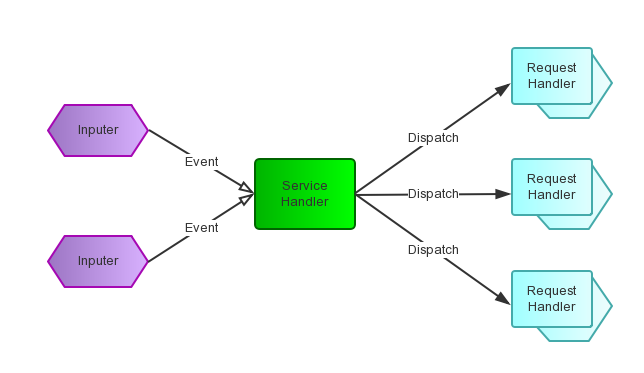
\includegraphics[scale = 0.7]{Reactor.png}
			\end{figure}
	
		从结构上,这有点类似生产者消费者模式,即有一个或多个生产者将事件放入一个Queue中,而一个或多个消费者主动的从这个Queue中Poll事件来处理;而Reactor模式则并没有Queue来做缓冲,每当一个Event输入到Service Handler之后,该Service Handler会主动的根据不同的Event类型将其分发给对应的Request Handler来处理。
		
		\subsection{例子学习ReActor}
			以一个餐饮为例,每一个人来就餐就是一个事件,他会先看一下菜单,然后点餐。就像一个网站会有很多的请求,要求服务器做一些事情。处理这些就餐事件的就需要我们的服务人员了。
			
			在多线程处理的方式会是这样的:
			一个人来就餐,一个服务员去服务,然后客人会看菜单,点菜。 服务员将菜单给后厨。
			二个人来就餐,二个服务员去服务……
			五个人来就餐,五个服务员去服务……
			
			这个就是\textbf{多线程的处理方式},\textbf{一个事件到来,就会有一个线程服务}。很显然这种方式在人少的情况下会有很好的用户体验,每个客人都感觉自己是VIP,专人服务的。如果餐厅一直这样同一时间最多来5个客人,这家餐厅是可以很好的服务下去的。
			
			来了一个好消息,因为这家店的服务好,吃饭的人多了起来。同一时间会来10个客人,老板很开心,但是只有5个服务员,这样就不能一对一服务了,有些客人就要没有人管了。老板就又请了5个服务员,现在好了,又能每个人都受VIP待遇了。
			
			越来越多的人对这家餐厅满意,客源又多了,同时来吃饭的人到了20人,老板高兴不起来了,再请服务员吧,占地方不说,还要开工钱,再请人就攒不到钱了。怎么办呢?老板想了想,10个服务员对付20个客人也是能对付过来的,服务员勤快点就好了,伺候完一个客人马上伺候另外一个,还是来得及的。综合考虑了一下,老板决定就使用10个服务人员的线程池啦
			
			但是这样有一个比较严重的缺点就是,如果正在接受服务员服务的客人点菜很慢,其他的客人可能就要等好长时间了。有些火爆脾气的客人可能就等不了走人了。
			
			\textbf{Reactor如何处理这个问题呢:}
			
			老板后来发现,客人点菜比较慢,大部服务员都在等着客人点菜,其实干的活不是太多。老板能当老板当然有点不一样的地方,终于发现了一个新的方法,那就是:当客人点菜的时候,服务员就可以去招呼其他客人了,等客人点好了菜,直接招呼一声“服务员”,马上就有个服务员过去服务。嘿嘿,然后在老板有了这个新的方法之后,就进行了一次裁员,只留了一个服务员!这就是\textbf{用单个线程来做多线程的事}。
			
				\begin{figure}[h]
					\centering
					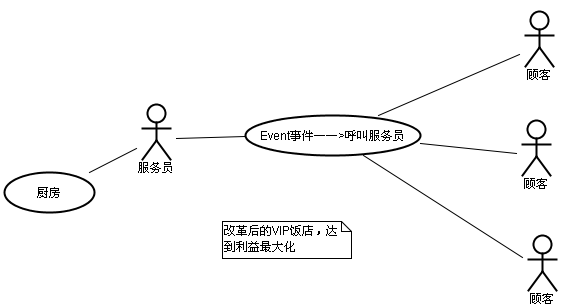
\includegraphics[scale = 0.8]{ReactorExample.png}
				\end{figure}
			
			实际的餐馆都是用的Reactor模式在服务。一些设计的模型其实都是从生活中来的。
			
			Reactor模式主要是提高系统的吞吐量,在有限的资源下处理更多的事情。
			
			在单核的机上,多线程并不能提高系统的性能,除非在有一些阻塞的情况发生。否则线程切换的开销会使处理的速度变慢。就像你一个人做两件事情,1、削一个苹果。2、切一个西瓜。那你可以一件一件的做,我想你也会一件一件的做。如果这个时候你使用多线程,一会儿削苹果,一会切西瓜,可以相像究竟是哪个速度快。这也就是说为什么在单核机上多线程来处理可能会更慢。
			
			但当有阻碍操作发生时,多线程的优势才会显示出来,现在你有另外两件事情去做,1、削一个苹果。2、烧一壶开水。我想没有人会去做完一件再做另一件,你肯定会一边烧水,一边就把苹果削了。
		
	\subsection{参考}
	\url{http://daimojingdeyu.iteye.com/blog/828696}
	
	\url{http://www.blogjava.net/DLevin/archive/2015/09/02/427045.html}	
	
	\section{阻塞IO服务器模型之单线程服务器模型}
		单线程服务器模型是最简单的一个服务器模型,几乎我们所有程序员在刚开始接触网络编程(不管是B/S结构还是C/S结构)都是从这个简单的模型开始。这种模型只提供同时一个客户端访问,多个客户端访问必须要等到前一个客户端访问结束,一个一个排队,即提供一问一答服务。
		\begin{figure}[h]
			\centering
			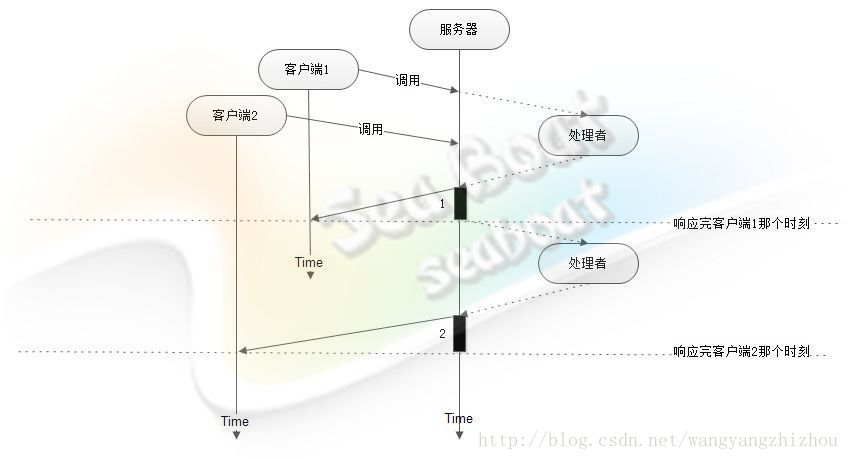
\includegraphics[scale = 1.6]{IO_SingleThread_Blocking.jpg}
			\caption{单线程阻塞服务器模型}
			\label{Blocking_Single}
		\end{figure}
	
		图\ref{Blocking_Single}展示了单线程阻塞服务器是怎样响应客户端的访问。首先,服务器必须初始化一个Serversocket实例,绑定某个端口号,并使之监听客户端的访问,以此提供一种服务。接着客户端1远程调用服务器的这个服务,服务器接受到请求后,对其进行处理,并返回信息给客户端1,整个过程都是在一个线程里面完成的。最后,就算客户端2在服务器处理完客户端1之前就进行请求访问,也要等服务器对客户端1响应完后,才会对客户端2进行响应处理。
		
		我们注意到,大部分的\verb|socket|操作都是阻塞的,所谓阻塞是指调用后不马上返回调用结果,而让当前线程一直阻塞,只有当该调用获得结果或者超时时才会返回。而我们的图2-6-1-1也有很多个节点都是阻塞的,例如,服务器阻塞监听客户端,直到有客户端访问才返回一个socket;对于客户端,建立一个socket连接后,也进行阻塞,直到服务器响应。几乎所有的IO操作都会产生阻塞,在网络编程中体现在socket的通信。这种阻塞给网络编程带来了一个问题,如图中黑块1和黑块2部分,当服务器处理完进行IO操作(这里的IO操作其实是给客户端发送消息)时,服务器必须要等到客户端成功接收才能继续往下处理另外一个客户端的请求,在此期间,线程将无法执行任何运算跟响应任何客户端请求。而如果这过程永远发送不到客户端,服务器就一直阻塞在那里了,不会接着处理任何事情。
		
		这种模型的特点是:最简单的服务器模型,整个运行过程都只有一个线程,只能支持同时处理一个客户端的请求,如果多个客户端访问必须排队等待,服务器系统资源消耗较小,但并发能力低,如果遇到IO操作出现错误异常将导致服务器停止运行,容错能力差。一般这种模型一般用在访问跟并发量少,请求是短暂的、无状态的,对响应时间要求不高,处理逻辑较复杂的场合。

	\section{ProActor}
	
	
	\section{Reactor with Proactor}
		以读取操作为例
		
		\subsection{reactor}
			\verb|Reactor|模式用于\verb|同步I/O|
			
			\begin{enumerate}
				\item 应用程序注册读就需事件和相关联的事件处理器
				\item 事件分离器等待事件的发生
				\item 当发生读就需事件的时候,事件分离器调用第一步注册的事件处理器
				\item 事件处理器首先执行实际的读取操作,然后根据读取到的内容进行进一步的处理
			\end{enumerate}
		
		\subsection{proactor}
			\verb|Proactor|运用于\verb|异步I/O|操作
			
			\begin{enumerate}
				\item 应用程序初始化一个异步读取操作,然后注册相应的事件处理器,此时事件处理器不关注读取就绪事件,而是关注读取完成事件,这是区别于\verb|Reactor|的关键。
				\item 事件分离器等待读取操作完成事件
				\item 在事件分离器等待读取操作完成的时候,操作系统调用内核线程完成读取操作,并将读取的内容放入用户传递过来的缓存区中。这也是区别于\verb|Reactor|的一点,\verb|Proactor|中,应用程序需要传递缓存区。
				\item 事件分离器捕获到读取完成事件后,激活应用程序注册的事件处理器,事件处理器直接从缓存区读取数据,而不需要进行实际的读取操作。
			\end{enumerate}
		
		\subsection{区别}
			\verb|Proactor|中写入操作和读取操作,只不过\textbf{感兴趣的事件是写入完成事件}
		
			\verb|Reactor和Proactor|模式的主要区别就是真正的读取和写入操作是有谁来完成的,\verb|Reactor|中需要应用程序自己读取或者写入数据,而\verb|Proactor|模式中,应用程序不需要进行实际的读写过程,它只需要从缓存区读取或者写入即可,操作系统会读取缓存区或者写入缓存区到真正的\verb|IO|设备.
	
	\section{半同步半异步模型}
		\subsection{同步}
			I/O 事件为就绪状态时 通知应用程序,数据的搬放由应用程序本身来完成,涉及应用缓存与内核缓存的复制效率问题。
			
		\subsection{异步}
			I/O 事件为完成状态时 通知应用程序,数据的搬放由内核来完成,通知时已将数据从缓存中读到应用缓存,或从应用写入内核缓存中,I/O 效率更高。
			
		\subsection{半同步半异步}
			\url{http://blog.csdn.net/zhuziyu1157817544/article/details/72486157}
			
			异步负责I/O事件 处理,同步负责处理用户逻辑
			
			\subsubsection{半同步半反应堆模式}
				\begin{figure}[h]
					\centering
					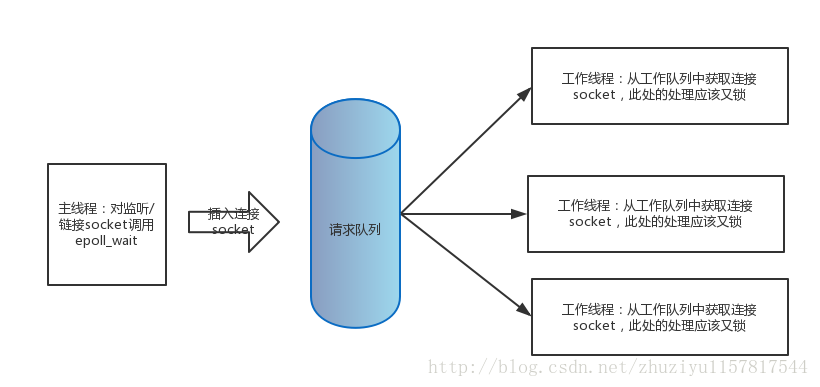
\includegraphics[scale = 0.5]{half.png}
					\caption{半同步半异步}
				\end{figure}
				
				\begin{itemize}
					\item \textbf{异步线程}只有一个,由主线程充当,\textbf{负责监听}所有\verb|socket|事件。
						\begin{enumerate}
							\item 如果监听\verb|socket|上有可读事件发生,指的是新的链接请求到来,那么异步线程接受它,往\verb|epoll|内核事件表中注册该\verb|socket|上的读写事件。
							\item 如果连接\verb|socket|上有读写事件发生,要么是新的客户请求,要么是有数据要发送给客户端,主线程就把改连接socket插入请求队列。
						\end{enumerate}
					
					\item 所有的\textbf{工作线程}睡眠在请求队列上,有任务来的时候,空闲线程竞争,获取任务接管权。此后,该线程管理这个\verb|socket|所有的I/O任务,直到客户关闭连接。
				\end{itemize}
				
				\subparagraph{缺点}\verb|->|
					\begin{itemize}[itemindent = 1em]
						\item 主线程和工作线程共享一个请求队列,因此一但队列中的任务有变更,就需要加锁保护
						\item 每一个工作线程在同一时间只能处理一个客户请求,对于客户数良多,但是工作任务少的情况下,队友很多任务堆积,客户的响应速度越来越慢
					\end{itemize}
				
				\subparagraph{例子}\verb|->| 
				
					\url{http://blog.csdn.net/u013074465/article/details/46357219}
			\subsubsection{more Efficient}
				\textbf{改进方面}:让一个工作线程能够处理很多的客户请求。即对每一个工作线程,对于各自连接的\verb|socket|们调用\verb|epoll_wait|。
				
				\begin{figure}[h]
					\centering
					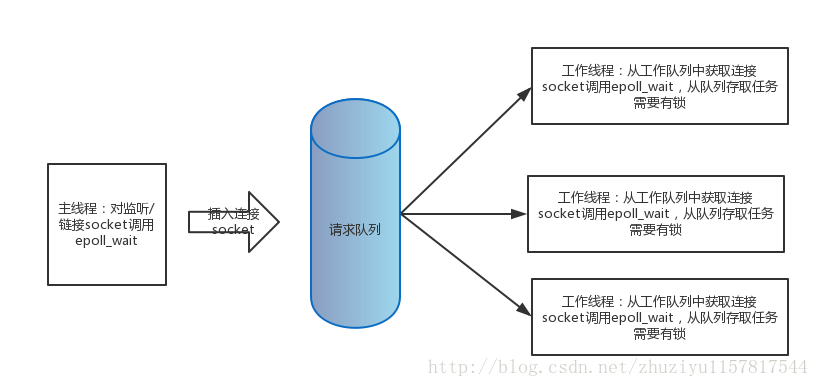
\includegraphics[scale = 0.5]{half2.png}
					\caption{半同步半异步-2}
				\end{figure}
	
	\section{领导者追随者模式}
		放风的山贼(领导者)与 睡觉(追随者)、抢劫(old领导者)的山贼
		
		\url{http://blog.csdn.net/jinchaoh/article/details/50427733}
	
\chapter{如何使用多台机器并行处理数据}
	\section{集群服务器}
			\textbf{同一个业务},部署在多个服务器上
			
			小饭店原来只有一个厨师,切菜洗菜备料炒菜全干。后来客人多了,厨房一个厨师忙不过来,又请了个厨师,两个厨师都能炒一样的菜,这两个厨师的关系是集群。为了让厨师专心炒菜,把菜做到极致,又请了个配菜师负责切菜,备菜,备料,厨师和配菜师的关系是分布式,一个配菜师也忙不过来了,又请了个配菜师,两个配菜师关系是集群
			
	\section{分布式服务器}
			\textbf{一个业务分拆多个子业务},部署在不同的服务器上,具体的平台有Hadoop.分布式 强调 机器间的协作,\textbf{其重点是任务可拆分}, 如 某个任务需要一个机器运行10个小时, 将该该任务用10台机器的分布式跑,可能2个小时就跑完了。(\textbf{子任务之间有依赖关系})。
\chapter{调试}
	\section{ACK 与 Seq}
		\subsection{建立与释放阶段}
			\begin{table}[htbp]
				\centering
				\caption{建立阶段演示}
				\begin{tabular}{m{1cm}|m{3cm}|m{4cm}|m{4cm}}
					\toprule
						序号 & 方向 & Seq & ACK \\
					\midrule
						 1& \verb|A -> B|& 10000 & 0 \\
						 2& \verb|B -> A|& 20000 & 10000+1 = 10001 \\
					 	 3& \verb|A -> B|& 10001 & 20000+1 = 20001 \\
					\bottomrule
				\end{tabular}
			\end{table}
			\begin{enumerate}
				\item \verb|A|向\verb|B|发起连接请求,以一个随机数初始化\verb|A|的\verb|seq|,这里假设为\verb|10000|,此时\verb|ACK=0|
				\item \verb|B|收到\verb|A|的连接请求后,也以一个随机数初始化\verb|B|的\verb|seq|,这里假设为\verb|20000|,意思是:你的请求我已收到,我这方的数据流就从这个数开始。\verb|B|的\verb|ACK|是\verb|A|的\verb|seq|加\verb|1|,即\verb|10000+1 = 10001|
				\item \verb|A|收到\verb|B|的回复后,它的\verb|seq|是它的上个请求的\verb|seq|加\verb|1|,即\verb|10000+1 = 10001|,意思也是:你的回复我收到了,我这方的数据流就从这个数开始。\verb|A|此时的\verb|ACK|是\verb|B|的\verb|seq|加\verb|1|,即\verb|20000+1=20001|
			\end{enumerate}
		
		\subsection{数据传输阶段}
			\begin{table}[htbp]
				\centering
				\caption{数据传输阶段演示}
				\begin{tabular}{m{1cm}|m{3cm}|m{4cm}|m{4cm}|m{1cm}}
					\toprule
						序号 & 方向 & Seq & ACK & Size\\
					\midrule
						1& \verb|A -> B|& 40000 & 70000 				&  1514 \\
						2& \verb|B -> A|& 70000 & 40000+1514-54 = 41460 &  54 \\
						3& \verb|A -> B|& 41460 & 70000+54-54 = 70000   &  1514 \\
						4& \verb|B -> A|& 70000 & 41460+1514-54 = 42920 &  54 \\
					\bottomrule
				\end{tabular}
			\end{table}
			\begin{enumerate}
				\item B接收到A发来的seq=40000,ack=70000,size=1514的数据包
				\item 于是B向A也发一个数据包,告诉B,你的上个包我收到了。B的seq就以它收到的数据包的ACK填充,ACK是它收到的数据包的SEQ加上数据包的大小(不包括以太网协议头,IP头,TCP头),以证实B发过来的数据全收到了。
				\item A在收到B发过来的ack为41460的数据包时,一看到41460,正好是它的上个数据包的seq加上包的大小,就明白,上次发送的数据包已安全到达。于是它再发一个数据包给B。这个正在发送的数据包的seq也以它收到的数据包的ACK填充,ACK就以它收到的数据包的seq(70000)加上包的size(54)填充,即ack=70000+54-54(全是头长,没数据项)。
			\end{enumerate}
			
		\subparagraph{Note}-
		
			\begin{lstlisting}
	1.如果对方没有数据过来,则自己的确认号不变,序列号为上次的序列号加上本次应用层数据发送长度.
	2.其实在握手和结束时确认号应该是对方序列号加1,传输数据时则是对方序列号加上对方携带应用层数据的长度.
			\end{lstlisting}
	\section{strace}
		\url{http://blog.csdn.net/zhouzhenhe2008/article/details/63687169}
		
		\begin{itemize}
			\item 每一行都是一次系统调用。
			\item 等号左边是系统调用函数及其参数,右边是返回值。
			\item 系统首先调用\verb|execve|开始一个新的进程,最后调用\verb|exit_group|退出进程,完成整个程序的执行过程。strace首先调用\verb|fork|或者\verb|clone|函数新建一个子进程,然后在子进程中调用\verb|exec|载入需要执行的程序。
			\item \verb|brk(0)   = 0x8803000|, 以0作为参数的调用\verb|brk|,返回值是内存管理的起始地址,如果程序调用调用\verb|malloc|,内存管理分配将从\verb|0x8803000|地址开始。
			\item \verb|access|是检查文件是否存在
			\item 使用\verb|mmap2|函数进行\textbf{匿名内存映射},以此来获取内存空间,\textit{其第二参数}就是需要获取内存空间的长度,返回值为内存空间的起始地址。
			
			匿名内存映射就是为了不涉及具体的文件名,避免了文件的创建和打开,只能用于具有亲缘关系的进程间通信。
		\end{itemize}
		
		\subsection{指定追踪类型}
			\verb|-e expr|
			
			指定一个表达式,用来控制如何跟踪
			
			\verb|-e trace=set |
			只跟踪指定的系统 调用.例如:-e trace=open,close,rean,write表示只跟踪这四个系统调用.默认的为set=all. 
			
			\verb|-e trace=file |
			只跟踪有关文件操作的系统调用. 
			
			\verb|-e trace=process |
			只跟踪有关进程控制的系统调用. 
			
			\verb|-e trace=network |
			跟踪与网络有关的所有系统调用. 
				\begin{figure}[h]
					\centering
					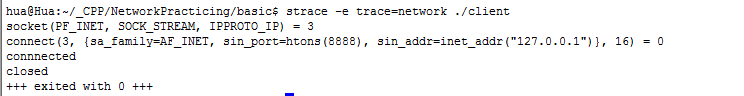
\includegraphics[scale = 0.6]{strace-Net.png}
				\end{figure}
				
			\verb|-e strace=signal |
			跟踪所有与系统信号有关的 系统调用 
			
			\verb|-e trace=ipc |
			跟踪所有与进程通讯有关的系统调用 
		
	\section{tcpdump}
	
	\section{nc}
	
	\section{lsof}lsof(list open files)是一个\textbf{列出当前系统打开文件的工具}
	
	\section{netstat}Netstat 命令用于显示各种网络相关信息,如网络连接,路由表,接口状态 (Interface Statistics),masquerade 连接,多播成员 (Multicast Memberships) 等等
	
	\section{vmstat}
	
	\section{ifstat}ifstat工具是个\textbf{网络接口监测工具},比较简单看网络流量
	
	\section{mpstat}mpstat是Multiprocessor Statistics的缩写,是实时系统监控工具。其报告与CPU的一些统计信息,这些信息存放在/proc/stat文件中。在多CPUs系统里,其不但能查看所有CPU的平均状况信息,而且能够查看特定CPU的信息。mpstat最大的特点是:\textbf{可以查看多核心cpu中每个计算核心的统计数据};而类似工具\textbf{vmstat只能查看系统整体cpu情况}。
	
	\section{top}
	
	\section{ping}
	
	\section{iptables}
	
	\section{TTCP}
		\url{http://www.feamane.org/comms/testtools/ttcp/ttcp-quickstartguide.html}
	
\chapter{理论}
	\section{网络的性能}
		\subsection{速率} 计算机中数据量的单位是用比特(\verb|bit|)来表示的,它是一个二进制数,\verb|0或者1|,网络中的速率是连接在计算机网络上的主机在数字信道上传送数据的速率,也可以说是数据率 或 比特率\verb|bit/s = bps(bit per second)|,当比特率较高时,就可以用\verb|Kb/s Mbs/s Gb/s|
		
		\subsection{带宽} 有两种含义,\textbf{第一种}是指某个信号具有的频带宽度,用赫兹表示(\verb|Hz|)。\textbf{第二种}就是我们说的计算机网络中使用的带宽,是通信线路所能传送数据的能力,\textbf{简洁的说是最高数据率}
		
		\subsection{吞吐量} 吞吐量(\verb|throughput|) 表示单位时间内通过某个网络(或者 信道、接口)的数据量。 吞吐量更经常地用于对现实世界中的网络的一种测量,以便知道实际上到底有多少数据量能够通过网络.
		
			吞吐量受网络的\textbf{带宽}或\textbf{网络的额定速率}的限制。对\verb|100Mb/s|的以太网,其典型的吞吐量可能只有\verb|70Mb/s|。
			
		\subsection{时延} 时延(\verb|delay| 或 \verb|latency|)是指数据(一个报文或分组,甚至比特) 从网络(或链路) 的一端传送到另一端 所需的时间。 它有时也称为 \textbf{延迟}或\textbf{迟延}.
			
			时延通常由以下几个方面组成:
			\subparagraph{发送时延 Transmission Delay} 是主机或路由器发送数据帧所需要的时间.. 也就是从发送数据帧的第一个比特算起,到该帧的最后一个比特发送完毕所需要的时间, 因此发送时延又称\textbf{传输时延},发送时延的计算公式如下
			
				$$ \verb|发送时延| = \verb|数据帧长度(b)| \div \verb|信道带宽(b/s)|$$
			
			由此可见,对于一定的网络.. 发送时延与发送的帧长成正比,与信道带宽成反比,而\textbf{并非是固定不变的}..
			
			\subparagraph{传播时延 Propagation Delay} 是电磁波在信道中传播一定的距离需要花费的时间..计算公式如下:
			
				$$ \verb|传播时延| = \verb|信道长度(m)| \div \verb|电磁波在信道上的传播速率(m/s)|$$
			
			\subparagraph{处理时延} 主机或路由器 在收到分组时 要处理一定的时间 进行处理,例如分析分组的首部、从分组中提取数据部分、进行差错检验或查找适当的路由等, 这就产生了 处理时延.
			
			\subparagraph{排队时延} 分组在经过网络传输时,要经过许多的路由器,但分组在进入路由器后要现在输入队列中排队等待处理. 在路由器确定了转发接口后,还要在 输出队列中 排队等待转发,这就产生了 排队时延.
			
			$$ \verb|总时延| = \verb|发送时延| + \verb|传播时延| + \verb|处理时延| + \verb|排队时延|$$
			
		\subsection{时延带宽积}
			\verb|时延带宽积 = 传播时延 × 带宽|,链路的\verb|时延宽带积| 又称为 \textbf{以比特为单位的链路长度}
			
		\subsection{往返时间RTT} 往返时间 \verb|RTT(Round-Trip Time)| 它表示从发送方发送数据开始,到发送方收到来自 接收方的确认 总共经历的时间.
				
		\subsection{利用率} 有信道利用率 和 网络利用率两种.. \textbf{信道利用率}指出谋信道有百分之几的时间是被利用的(有数据通过),完全空闲的信道利用率是0.  \textbf{网络利用率}则是全网络的信道利用率的加权平均值.  信道利用率并非越高越好, 这就跟高速公路一样.. 车流量大了..在某些地方就会出现堵塞,会增加行车时间..也就是网络时延.. 
		
		所以,\textbf{信道或网络利用率 过高会产生非常大的 时延}.
	\section{应用层 }
		\subsection{域名系统 DNS}
			域名系统(\verb|Domain Name System|缩写\verb|DNS,Domain Name|被译为域名)是因特网的一项核心服务,它作为可以\textbf{将域名}和\verb|IP|\textbf{地址}相互映射的一个\textbf{分布式数据库},能够使人更方便的访问互联网,而不用去记住能够被机器直接读取的\verb|IP数串|
			
			即将易记的域名\verb|www.baidu.com| 转换为 计算机识别的\verb|IP|地址\verb|192.168.2.1|
			\begin{figure}[h]
				\centering
				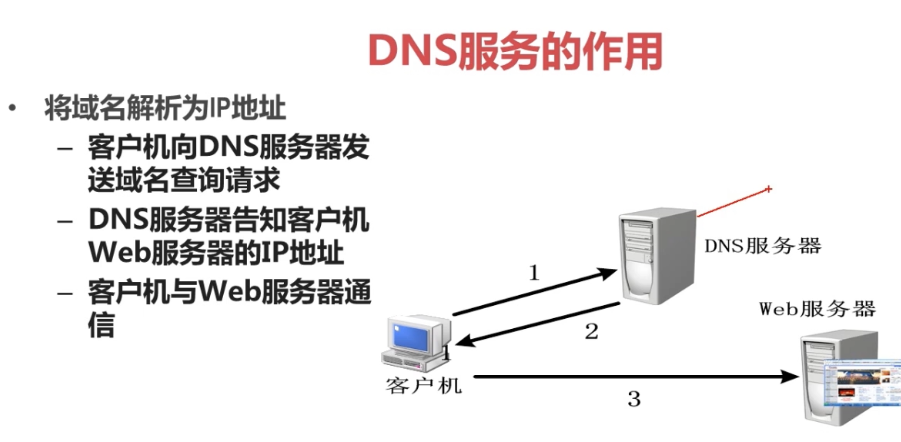
\includegraphics[scale=0.5]{DNS.png}
			\end{figure}
			
		\subsection{文件传送 FTP}
			\verb|FTP 是File Transfer Protocol|(文件传输协议)的英文简称,而中文简称为“\textbf{文传协议}”。用于\verb|Internet|上的控制文件的双向传输。同时,它也是一个应用程序(\verb|Application|)。
			
			基于不同的操作系统有不同的\verb|FTP|应用程序,而所有这些应用程序都遵守同一种协议以传输文件。在FTP的使用当中,用户经常遇到两个概念:"下载"(\verb|Download|)和"上传"(\verb|Upload|)。"下载"文件就是从远程主机拷贝文件至自己的计算机上;"上传"文件就是将文件从自己的计算机中拷贝至远程主机上。
			
		\subsection{万维 WWW}
			\verb|WWW|是环球信息网的缩写,(亦作“Web”、“WWW”、“'W3'”,英文全称为“\verb|World Wide Web|”),中文名字为“万维网”,"环球网"等,常简称为\verb|Web|。 \textbf{分为}\verb|Web客户端和Web服务器程序|。
			
			 \verb|WWW|\textit{可以让}\textbf{Web客户端}(常用浏览器)\textbf{访问浏览Web服务器上的页面}。 是一个由许多互相链接的超文本组成的系统,通过互联网访问。在这个系统中,每个有用的事物,称为一样“资源”;并且由一个全局“统一资源标识符”(\verb|URI|)标识;这些资源通过超文本传输协议(\verb|Hypertext Transfer Protocol|)传送给用户,而后者通过点击链接来获得资源。
		
		\subsection{动态主机配置 DHCP}
			\verb|DHCP(Dynamic Host Configuration Protocol,动态主机配置协议)|是一个局域网的网络协议,使用\verb|UDP|协议工作, 主要有两个用途:\textbf{给内部网络}或网络服务供应商\textbf{自动分配}\verb|IP|\textbf{地址},\textbf{给用户}或者内部网络管理员\textbf{作为对所有计算机作中央管理的手段}
		
		\subsection{电子邮件 SMTP IMAP}	
		
		\subsection{简单网络管理 SNMP}
		
		\subsection{APP 分别使用传输层的 协议对照}
			\begin{figure}[h]
				\centering
				\includegraphics[scale = 0.7]{App-Proposal.png}
			\end{figure}
		
	\section{传输层 TCP}		
		\subsection{基本概念对照} 
			\subsubsection{TCP 可靠性}
				在一个TCP连接中,仅有两方进行彼此通信。其可靠性的保证由以下措施完成
				
				\begin{enumerate}
					\item \textbf{数据块分割}:\textbf{应用数据被分割}成TCP认为最适合发送的数据块。这和\verb|UDP|完全不同,\textbf{应用程序产生的数据报长度将保持不变}。由TCP传递给IP的信息单位称为\textbf{报文段或段}(segment)
					
					\item \textbf{自适应的超时重传策略}:当TCP发出一个段后,它启动一个定时器,等待目的端确认收到这个报文段。如果不能及时收到一个确认,将重发这个报文段。
					
					\item 当TCP收到发自TCP连接另一端的数据,它将发送一个确认。这个确认不是立即发送,通常将推迟几分之一秒.
					
					\item \textbf{检验和}:TCP将保持它首部和数据的检验和。这是一个端到端的检验和,目的是检测数据在传输过程中的任何变化。如果收到段的检验和有差错, TCP将丢弃这个报文段和不确认收到此报文段(希望发端超时并重发)
					
					\item \textbf{数据有序}:既然TCP报文段作为IP数据报来传输,而IP数据报的到达可能会失序,因此TCP报文段的到达也可能会失序。如果必要, TCP将对收到的数据进行重新排序,将收到的数据以正确的顺序交给应用层。
					
					\item \textbf{丢弃重复数据}: 既然IP数据报会发生重复, TCP的接收端必须丢弃重复的数据。
					
					\item \textbf{流量控制}:TCP连接的每一方都有固定大小的缓冲空间。TCP的接收端只允许另一端发送接收端缓冲区所能接纳的数据。这将防止较快主机致使较慢主机的缓冲区溢出。
				\end{enumerate}
				
			\subsubsection{复用与分用}
				假定一个机关的 所有部门向外 单位发出的 公文都由 收发室负责寄出,这相当于各部门都“复用” 这个收发室。 当收发室收到从外单位寄出的公文时,则要完成“分用” 功能,即按照信封上写明的本机关的部门地址把公文正确进行交付
				
				运输层的\verb|复用和分用|功能也是类似的。 应用层所有的应用进程都可以通过运输层再传送到\verb|IP|层,这就是\textbf{复用}。 运输层从\verb|IP|层收到数据后必须交付给指明的应用进程,这就是\textbf{分用}。如下图\ref{MM}所示:
				
				\begin{figure}[h]
					\centering
					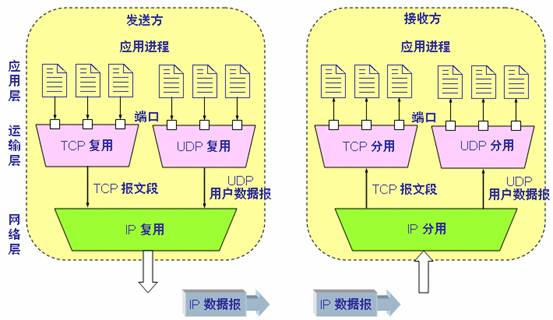
\includegraphics[scale = 0.8]{TCP-MM.jpg}
					\caption{分用复用图}
					\label{MM}
				\end{figure}
	
			\subsubsection{端口}
				\subparagraph{引入问题}
					运行在计算机中的进程是用进程标识符来标志的。但运行在应用层的各种应用进程却不应当让计算机操作系统指派它的进程标识符。这是因为在因特网上使用的计算机的操作系统种类很多,而不同的操作系统又使用不同格式的进程标识符,因此发送方非常可能无法识别其他机器上的进程。为了使运行不同操作系统的计算机的应用进程能够互相通信,就必须用统一的方法对 \verb|TCP/IP|体系的应用进程进行标志。而且由于进程的创建和撤销都是动态的,有时我们会改换接收报文的进程,但并不需要通知所有发送方。还有在实际应用中我们往往需要利用目的主机提供的功能来识别终点,而不需要知道实现这个功能的进程。
				
				\subparagraph{解决方法}
					解决这个问题的方法就是在运输层使用\textbf{协议端口号}(\verb|protocolport number|),或通常简称为端口(\verb|port|),端口用一个\verb|16|位端口号进行标志。端口号\textbf{只具有本地意义},即端口号只是为了标志本计算机应用层中的各进程。\textbf{在因特网中不同计算机的相同端口号是没有联系的}。虽然通信的终点是应用进程,但我们可以把端口想象是通信的终点,因为我们只要把要传送的报文交到目的主机的某一个合适的目的端口,剩下的工作(即最后交付目的进程)就由\verb|TCP|来完成
				
				\subparagraph{端口号分类}
					\begin{enumerate}[fullwidth,itemindent = 2em,label=(\arabic*)]
						\item \textbf{服务器端使用的端口号} 这里又分为两类
							\begin{itemize}[itemindent = 3em]
								\item \textbf{熟知端口号}或\textbf{系统端口号}:\verb|0~1023|,\verb|IANA| 把这些端口号指派给了\verb|TCP/IP| 最重要的一些应用程序.
									\begin{table}[H]
										\centering
										\begin{tabular}{|c|c|c|c|c|c|c|c|c|}
											\hline
											应用程序  & \verb|FTP| & \verb|TELNET| & \verb|SMTP| & \verb|DNS| & \verb|TFTP| & \verb|HTTP| & \verb|腾讯QQ| & \verb|MSSQL Server| \\
											\hline
											熟知端口号   & \verb|21| & \verb|23| & \verb|25| & \verb|53| & \verb|69| & \verb|80| & \verb|UDP8000| & \verb|5000| \\
											\hline
										\end{tabular}
									\end{table}
								\item \textbf{登记端口号}: \verb|1024~49151|
							\end{itemize}
						\item \textbf{客户端使用的端口号}: \verb|49152~65535| 
					\end{enumerate} 
		\subsection{UDP}
			\subsubsection{特点}
				\begin{itemize}
					\item \textbf{无连接}:在发送数据前不需要建立连接,当然发送数据结束完后也没有连接可释放,因此减少了 开销和发送数据之前的时延.
					\item \textbf{尽最大努力交付}:即不保证可靠交付
					\item \textbf{面向报文}:\verb|UDP| 对应用层交下来的 报文即不合并,也不拆分,而是保留这些报文的边界。也就是说,应用层交给\verb|UDP| 多长的报文,\verb|UDP| 就照样发送,即一次发送一个报文。
				\end{itemize}
			\subsubsection{网络控制特点}
				\begin{itemize}
					\item \textbf{UDP 没有拥塞控制}: 在网络出现堵塞也不会使源主机的发送速率降低.
					\item \textbf{UDP 支持1对1, 1对多, 多对1, 多对多}
					\item \textbf{UDP 的首部开销小}: 只有\verb|8|个字节,比\verb|TCP| 的\verb|20|个字节的首部要短
				\end{itemize}
		\subsection{TCP}
		
		
	\section{网络层 IP}
		\subsection{分类的IP地址}
			现在的\verb|IP|网络使用32位地址,以点分十进制表示,如\verb|172.16.0.0|。地址格式为:\verb|IP地址=网络地址+主机地址| 或 \verb|IP地址=主机地址+子网地址+主机地址|
			
			\subsubsection{IP 地址类型}
				\subparagraph{A类IP 地址}
					一个\verb|A类IP地址|由\verb|1字节|的\textbf{网络地址}和\verb|3字节|\textbf{主机地址}组成,网络地址的最高位必须是“\verb|0|”, \textbf{地址范围}从\verb|1.0.0.0| 到\verb|126.0.0.0|。可用的\verb|A类网络|有$2^7 - 2(\verb|全0 与 127|)$\verb|共126|个,每个网络能容纳\verb|1亿多个|主机
					
				\subparagraph{B类IP 地址}
					一个\verb|B类IP地址|由\verb|2字节|的\textbf{网络地址}和\verb|2字节|的\textbf{主机地址}组成,网络地址的最高位必须是“\verb|10|”,地址范围从\verb|128.0.0.0|到\verb|191.255.255.255|。可用的\verb|B类网络|有$2^{14} - 1(\verb|全0|)$\verb|16382|个,每个网络能容纳\verb|6万多个|主机
					
				\subparagraph{C类IP 地址}
					一个\verb|C类IP地址|由\verb|3字节|的\textbf{网络地址}和\verb|1字节|的\textbf{主机地址}组成,网络地址的最高位必须是“\verb|110|”。范围从\verb|192.0.0.0|到\verb|223.255.255.255|。\verb|C类网络|可达\verb|209万余|个,每个网络能容纳\verb|254个|主机
				
					\begin{figure}[h]
						\centering
						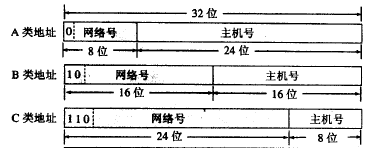
\includegraphics[scale = 0.9]{IPClassify.png}
					\end{figure}
					
					\begin{table}[H]
						\centering
						\caption{\textbf{IP 地址的指派范围}}
						\begin{tabular}{|c|m{3cm}|m{3cm}|m{3cm}|m{3cm}|}
							\hline 
							网络类别 & 最大可指派的网络数 & 第一个可指派的网络号 & 最后一个可指派的网络号 & 每个网络中最大的主机数\\
							\hline
							\verb|A |&$126(2^7 - 2) $ & \verb|1| & \verb|126| & \verb|16777214|\\
							\verb|B |&$16383(2^{14} - 1) $ & \verb|128.1| & \verb|191.255| & \verb|65534|\\
							\verb|C |&$2097151(2^{21} - 1) $ & \verb|192.0.1| & \verb|223.255.255| & \verb|254|\\
							\hline
						\end{tabular}
					\end{table}
					
					\begin{table}[H]
						\centering
						\caption{\textbf{一般不使用的IP 地址}}
						\begin{tabular}{|c|m{3.1cm}|c|c|m{7cm}|}
							\hline 
							网络号 & 主机号 & 源地址使用 & 目的地址使用 & 代表的意思\\
							\hline
							\verb|0 |&\verb|0 | & \verb|可以| & \verb|不可| & \verb|在本网络上的本主机| \\
							\verb|0 |&\verb|host-id | & \verb|可以| & \verb|不可| & \verb|在本网络上的某个主机host-id| \\
							\verb|全1 |&\verb|全1 | & \verb|不可| & \verb|可以| & \verb|只在本网络上进行广播(各路由器均不转发)| \\
							\verb|net-id|&\verb|全1 | & \verb|不可| & \verb|可以| & \verb|对net-id 上的所有主机进行广播| \\
							\verb|127 |&\verb|非全0或全1的任何数| & \verb|可以| & \verb|不可以| & \verb|用于本地软件环回测试之用| \\
							\hline
						\end{tabular}
					\end{table}
				\subparagraph{其他} 全零(“\verb|0.0.0.0|”)地址对应于\textbf{当前主机}。全“1”的IP地址(“\verb|255.255.255.255|”)是\textbf{当前子网的广播地址}。数字\verb|127|保留给\textbf{内部回环函数}
					
		\subsection{子网掩码}
			子网掩码(\verb|subnet mask|)又叫网络掩码、地址掩码、子网络遮罩,它是一种用来指明一个\verb|IP|地址的哪些位标识的是主机所在的子网,以及哪些位标识的是主机的位掩码。子网掩码不能单独存在,它必须结合\verb|IP|地址一起使用。\textbf{子网掩码}只有一个作用,就是\textbf{将}某个\verb|IP|地址\textbf{划分成}\textit{网络地址}\textbf{和}\textit{主机地址}两部分
				
			子网掩码——屏蔽一个\verb|IP|地址的网络部分的“全1”比特模式。对于\textbf{A类地址}来说,默认的子网掩码是\verb|255.0.0.0|;对于\textbf{B类地址}来说默认的子网掩码是\verb|255.255.0.0|;对于\textbf{C类地址}来说默认的子网掩码是\verb|255.255.255.0|
				
			\textbf{利用}子网掩码\textbf{可以}\textit{把大的网络划分成子网},\textbf{也可以}把小的网络\textbf{归并成}大的网络即超网
			
			注意,不同的网络类型(ABC)也可以使用比其小的子网掩码,如B类地址使用C类子网掩码.
			如\begin{figure}[h]
				\centering
				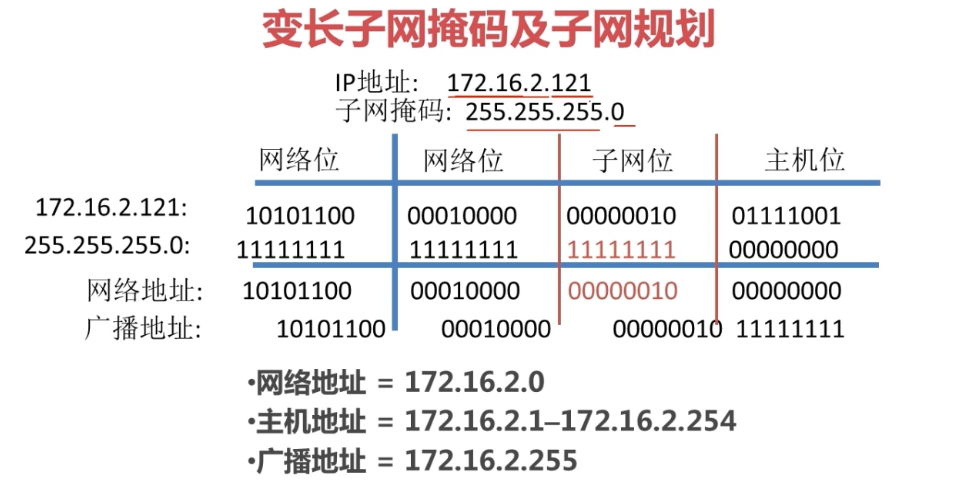
\includegraphics[scale = 0.5]{subNetMask.png}
			\end{figure}
			
	\section{数据链路层 Hardware}
	
	
	
\chapter{资源}    
\section{读书路线}
	\subparagraph{0.Linux 命令大全}
	\subparagraph{1.Linux高性能服务器编程}
	\subparagraph{2.构建高可用Linux服务器}
	\subparagraph{3.Linux多线程服务端编程}
\section{项目学习}
	\subparagraph{参见 C++\_Project}
		\begin{itemize}[itemindent = 1em]
			\item muduo
			\item nginx
			\item libevent
			\item lighttpd
		\end{itemize}
\section{参考}
    \subparagraph{0.学习路线}\url{http://www.cnblogs.com/lizhanwu/p/4164456.html}
	\subparagraph{1.使用socket通信实现FTP服务器}\url{http://www.ibm.com/developerworks/cn/linux/l-cn-socketftp/}
	\subparagraph{2.游戏服务器的见闻}\url{http://blog.sina.com.cn/s/blog_55d572ca0100uvzt.html}
	\subparagraph{3.高性能服务器模型}\url{http://blog.csdn.net/zs634134578/article/details/19806429}
	\subparagraph{4.面试题} \url{http://blog.csdn.net/chencheng126/article/details/44407901}
	
		\url{http://blog.chinaunix.net/uid-29087962-id-3988587.html}
	
	\subparagraph{5.相关函数} \url{http://blog.csdn.net/caianye/article/details/8598051}
\end{document} 
 		    